\documentclass [MS] {uclathes}
\usepackage{bm}
\usepackage{color}
\usepackage{float}
\usepackage{amsthm}
\usepackage{xcolor}
\usepackage{amsmath}
\usepackage{amssymb}
\usepackage{comment}
\usepackage{environ}
\usepackage{wrapfig}
\usepackage{amsfonts}
\usepackage{etoolbox}
\usepackage{fancyhdr}
\usepackage{graphicx}
\usepackage[papersize={8.5in,11in}]{geometry}
\usepackage{hyperref}
\usepackage{lettrine}
\usepackage{mdframed}
\usepackage{multirow}
% \usepackage{algorithm2e}
\usepackage{algorithm,algpseudocode}
\usepackage{subcaption}
\usepackage{indentfirst}
\usepackage[shortlabels]{enumitem}
\usepackage{siunitx}
\usepackage{tabularx}
\hypersetup{
    colorlinks=true,
    linkcolor=blue,
    filecolor=magenta,      
    urlcolor=blue,
}
% \input {mymacros}                         % personal LaTeX macros

%%%%%%%%%%%%%%%%%%%%%%%%%%%%%%%%%%%%%%%%%%%%%%%%%%%%%%%%%%%%%%%%%%%%%%
%
% Usually things live in separate flies.
%
% \input {prelim}                           % preliminary page info

%%%%%%%%%%%%%%%%%%%%%%%%%%%%%%%%%%%%%%%%%%%%%%%%%%%%%%%%%%%%%%%%%%%%%%%%
%                                                                      %
%                          PRELIMINARY PAGES                           %
%                                                                      %
%%%%%%%%%%%%%%%%%%%%%%%%%%%%%%%%%%%%%%%%%%%%%%%%%%%%%%%%%%%%%%%%%%%%%%%%

% \title          {Multi-Agent Interaction and Deflection \\
%                  with Tumbling Objects in Orbit}
                 
% \author         {Aaron John Sabu}
% \department     {Electrical and Computer Engineering}
% Note:  degreeyear should be optional, but as of  5-Feb-96
% it seems required or you get a year of ``2''.   -johnh
% \degreeyear     {2023}

%%%%%%%%%%%%%%%%%%%%%%%%%%%%%%%%%%%%%%%%%%%%%%%%%%%%%%%%%%%%%%%%%%%%%%%%

% \chair          {Paulo Tabuada}
% \member         {Brett T.\ Lopez}
% \member         {Bahman Gharesifard}

%%%%%%%%%%%%%%%%%%%%%%%%%%%%%%%%%%%%%%%%%%%%%%%%%%%%%%%%%%%%%%%%%%%%%%%%

% \dedication     {\textsl{To God Almighty \\
%                 for picking the right neurons in my brain \\
%                 to picking the right transistors on my laptop}}

%%%%%%%%%%%%%%%%%%%%%%%%%%%%%%%%%%%%%%%%%%%%%%%%%%%%%%%%%%%%%%%%%%%%%%%%

\acknowledgments {The extent of knowledge I have received under the guidance of Brett is unmeasurable, be it regarding insight into the technique of tube model predictive control or into fixing the annoying simulation errors.
However, it is just as true to state how supportive Brett has been as an advisor in how he understands personal situations and provides suggestions accordingly.
This is supplemented by the amount of insight he has provided into the idea of writing publications and theses.
I am deeply grateful for the invaluable contributions of my co-advisor, Dr. Paulo Tabuada, and my committee member, Dr. Bahman Gharesifard in my research and the completion of this thesis.
I particularly appreciate their unwavering patience and understanding, as my research endeavors encountered several unforeseen delays and setbacks.

I am forever grateful to my parents, Sabu John and Jessy Sabu John, who have supported me in my academic journey with every physical, mental, and emotional resource they could offer.
Without their constant encouragement to dare to reach beyond perceived limitations and chase my dreams, I would not stand where I do today.
My successes are a testament to their unwavering dedication, my flaws tempered by their unconditional love.
This extends to my amazing sister, Priscilla Sabu Ajin, who, despite all of my shenanigans, has been there for me as a never-ending source of encouragement.

My labmates, especially Helene Levy, Samuel Gessow, David Thorne, and Sarah Enayati have been extremely supportive in helping me realize what makes up for relevant research.
This extends to my former labmates, Kenny Chen and Ryan Nemiroff who have been there for me since my first quarter here at UCLA.
I cherish the invaluable lessons and intellectual engagement provided by my close friend, Alexander Thoms.
He has consistently challenged my thinking and kept my mind ``locked in," inspiring me to continuously strive for growth.
Similarly, I am deeply grateful to my dearest friend, Robert Kowalski, whose introduction to the fascinating world of powerlifting has provided much-needed solace and balance, reminding me of the joy found in physical pursuits.

And above all, thank God for helping me get where I am and for being my sure foundation for the future ahead! Soli Deo Gloria!
}


%%%%%%%%%%%%%%%%%%%%%%%%%%%%%%%%%%%%%%%%%%%%%%%%%%%%%%%%%%%%%%%%%%%%%%%%

% \vitaitem   {1974--1975}
%                 {Campus computer center ``User Services'' programmer and
%                 consultant, Stanford Center for Information Processing,
%                 Stanford University, Stanford, California.}
% \vitaitem   {1974--1975}
%                 {Programmer, Housing Office, Stanford University.
%                 Designed a major software system for assigning
%                 students to on-campus housing.
%                 With some later improvements, it is still in use.}
% \vitaitem   {1975}
%                 {B.S.~(Mathematics) and A.B.~(Music),
%                 Stanford University.}
% \vitaitem   {1977}
%                 {M.A.~(Music), UCLA, Los Angeles, California.}
% \vitaitem   {1977--1979}
%                 {Teaching Assistant, Computer Science Department, UCLA.
%                 Taught sections of Engineering 10 (beginning computer
%                 programming course) under direction of Professor Leon
%                 Levine.
%                 During summer 1979, taught a beginning programming
%                 course as part of the Freshman Summer Program.}
% \vitaitem   {1979}
%                 {M.S.~(Computer Science), UCLA.}
% \vitaitem   {1979--1980}
%                 {Teaching Assistant, Computer Science Department, UCLA.}
% \vitaitem   {1980--1981}
%                 {Research Assistant, Computer Science Department, UCLA.}
% \vitaitem   {1981--present}
%                 {Programmer/Analyst, Computer Science Department, UCLA.}

%%%%%%%%%%%%%%%%%%%%%%%%%%%%%%%%%%%%%%%%%%%%%%%%%%%%%%%%%%%%%%%%%%%%%%%%

% \publication    {\textsl{MADHOUS Reference Manual.}
%                 Stanford University, Dean of Student Affairs
%                 (Residential Education Division), 1978.
%                 Technical documentation for the MADHOUS
%                 software system used to assign students to
%                 on-campus housing.}

%%%%%%%%%%%%%%%%%%%%%%%%%%%%%%%%%%%%%%%%%%%%%%%%%%%%%%%%%%%%%%%%%%%%%%%%

% \abstract{
In this thesis, we will address the problem of capturing a tumbling, i.e., noncooperative, object in orbit. A tumbling object, also known as the target, can be a malfunctioning satellite or space debris that must be stabilized or removed to prevent collisions with other surrounding assets. Typical approaches use agents, called chasers, that attach to the tumbling object to stabilize or change the target’s orbit. While rendezvous and docking with cooperative objects has been possible since Project Gemini in the 1960s, effective strategies for tumbling objects that account for uncertainty in the target’s orbit have yet to be developed. We propose a novel adaptive tube model predictive control (MPC) formulation that is composed of a rendezvous (initial approach) and docking phase with the target. Importantly, the formulation includes uncertainty in the eccentricity and the drag parameters of the target's orbit. The approach is able to ensure all safety constraints are satisfied while also being able to incorporate online data to improve the prediction model, resulting in less conservative behavior. Simulation results of a single chaser-target scenario illustrate the approach. Moreover, an optimization-based method is proposed for computing the optimal amount of thrust to stop the tumble of the target once the chaser has docked with the target. A multi-chaser strategy is also explored.
}

%%%%%%%%%%%%%%%%%%%%%%%%%%%%%%%%%%%%%%%%%%%%%%%%%%%%%%%%%%%%%%%%%%%%%%%%


%
% thesis_macros
% Copyright (C) 1995 by John Heidemann, <johnh@isi.edu>
%

% \RequirePackage{johnh_general}

\RequirePackage{ifthen}

% \def\epsfreduction{0.667}
\def\epsfgraphreduction{0.9}

% \newcommand\comment[1]{{[\sffamily #1]}}

%
% TeX seems to want to indent after chapters,
% although it shouldn't.  Rather than argue
% with it, I work around it manually by putting this
% hack in the right places:
\newcommand{\noindenthack}{\noindent}


\newcommand{\fwling}{featherweight layering}
\newcommand{\fwls}{featherweight layers}
\newcommand{\fwl}{featherweight layer}

\newcommand{\Fwling}{Featherweight layering}
\newcommand{\Fwls}{Featherweight layers}
\newcommand{\Fwl}{Featherweight layer}

\newcommand{\FwLing}{Featherweight Layering}
\newcommand{\FwLs}{Featherweight Layers}
\newcommand{\FwL}{Featherweight Layer}

\newcommand{\xvop}[2]{{\scomputer {{#1}\_{#2}}}}
\newcommand{\vop}[1]{\xvop{vop}{#1}}

\newcommand{\usec}{$\mu$seconds}
\newcommand{\unix}{Unix}

\newcommand{\dotdot}{\scomputer{..}}

\newenvironment{mycode}%
	{\small
	}{%
	}

\newcommand{\mylangle}{\langle}
\newcommand{\myrangle}{\rangle}
\newcommand{\myrightarrow}{\rightarrow}


%
% Sizes of various things:
%
  \newcommand{\tablesize}{\normalsize}
  \newcommand{\computertablesize}{\small}
  \newcommand{\bibliographysize}{\normalsize}

  %
  % Another space-saver:  shrink the figures and graphs.
  %
 \def\epsfreduction{0.85}
 \def\epsfgraphreduction{0.9}   % should be left at 0.9 with two-column text
% \def\epsfsize#1#2{\epsfreduction#1}

%\newcommand{\appendixnumbering}{
%	\renewcommand{\thechapter}{\Alph{chapter}}
%	\setcounter{chapter}{0}
%	}

\newenvironment{functions}%
	{\begin{description}}%
	{\end{description}}

\makeatletter
  \newcommand{\SubmitSingleSpace}{
    \ifissubmit
      \renewcommand\baselinestretch{\@singlespacing}\@normalsize
    \fi
  }
  \newcommand{\SubmitDoubleSpace}{
    \ifissubmit
      \renewcommand\baselinestretch{\@doublespacing}\@normalsize
    \fi
  }
\makeatother


\iffalse
Figure drawing style guide:

layer labels:
	helvetica 12pt bold
	(short acronyms) helvetica 14pt bold

spacing:  8 pixels
each layers will be 3 high and 7 or 7.5 wide

or spacing: 8 pts
each layer will be 4 high and 10 wide

boxes and vnode links are line #2
\fi



\begin{document}


%
% Title pages of the thing
% Copyright (C) 1995 by John Heidemann, <johnh@isi.edu>.
%



\title          {Capturing Tumbling Objects in Orbit \\
                 with Adaptive Tube Model Predictive Control}
                 
\author         {Aaron John Sabu}
\department     {Electrical and Computer Engineering}
\degreemonth    {September}
% Note:  degreeyear should be optional, but as of  5-Feb-96
% it seems required or you get a year of ``2''.   -johnh
\degreeyear     {2023}

%%%%%%%%%%%%%%%%%%%%%%%%%%%%%%%%%%%%%%%%%%%%%%%%%%%%%%%%%%%%%%%%%%%%%%%%

\chair          {Paulo Tabuada}
\chair          {Brett T. Lopez}
\member         {Bahman Gharesifard}
% \member         {Richard L.\ Baker}
% \member         {Robert M.\ Stevenson}

%%%%%%%%%%%%%%%%%%%%%%%%%%%%%%%%%%%%%%%%%%%%%%%%%%%%%%%%%%%%%%%%%%%%%%%%

% \dedication     {}

%%%%%%%%%%%%%%%%%%%%%%%%%%%%%%%%%%%%%%%%%%%%%%%%%%%%%%%%%%%%%%%%%%%%%%%%

% \acknowledgments {(Acknowledgments omitted for brevity.)}

%%%%%%%%%%%%%%%%%%%%%%%%%%%%%%%%%%%%%%%%%%%%%%%%%%%%%%%%%%%%%%%%%%%%%%
%
% vita
%
% \vitaitem{1968}{B.S., Computer Science, Caribou University}
% \vitaitem{etc.}{etc.}
% \vitaitem{1995}{Graduated, UCLA}

%%%%%%%%%%%%%%%%%%%%%%%%%%%%%%%%%%%%%%%%%%%%%%%%%%%%%%%%%%%%%%%%%%%%%%
%
% publications
%

% \publication{
% 	Richard~G.\ Guy, John~S.\ Heidemann, Wai Mak, Thomas~W.\ Page,~Jr.,\ 
% 	  Gerald~J.\ Popek, and Dieter Rothmeier.
% 	Implementation of the Ficus
% 	  replicated file system.
% 	In \emph{USENIX Conference Proceedings}, pages
% 	  63--71.
% 	USENIX, June 1990.
% }

% \publication{
% 	etc.
% }

%%%%%%%%%%%%%%%%%%%%%%%%%%%%%%%%%%%%%%%%%%%%%%%%%%%%%%%%%%%%%%%%%%%%%%

\abstract{
In this thesis, we will address the problem of capturing a tumbling, i.e., noncooperative, object in orbit. A tumbling object, also known as the target, can be a malfunctioning satellite or space debris that must be stabilized or removed to prevent collisions with other surrounding assets. Typical approaches use agents, called chasers, that attach to the tumbling object to stabilize or change the target’s orbit. While rendezvous and docking with cooperative objects has been possible since Project Gemini in the 1960s, effective strategies for tumbling objects that account for uncertainty in the target’s orbit have yet to be developed. We propose a novel adaptive tube model predictive control (MPC) formulation that is composed of a rendezvous (initial approach) and docking phase with the target. Importantly, the formulation includes uncertainty in the eccentricity and the drag parameters of the target's orbit. The approach is able to ensure all safety constraints are satisfied while also being able to incorporate online data to improve the prediction model, resulting in less conservative behavior. Simulation results of a single chaser-target scenario illustrate the approach. Moreover, an optimization-based method is proposed for computing the optimal amount of thrust to stop the tumble of the target once the chaser has docked with the target. A multi-chaser strategy is also explored.
}

%
% I built a custom title page to do what I want.  So sue me.
% NEEDSWORK:  I had to copy some stuff from uclathti.sty.
%
\makeatletter
  \newcommand{\CustomTitlePage}{
    \begin{titlepage}
      \ColumnSave
      \vspace*{1.5in}   % a hacky way to center.  TeX didn't like \vfill.
      \begin{center}
  
      {\bfseries\huge \@title} \\
      \vskip 48pt plus0pt minus18pt
  
      {\large \@author} \\
      \vskip 12pt plus0pt minus3pt
      {\large University of California, Los Angeles} \\
      \vskip 6pt plus0pt minus2pt
      {\large \@degreemonth, \@degreeyear} \\
      \vskip 48pt plus0pt minus18pt
  
      \normalsize A \@thesisname\
      submitted in partial satisfaction \\
      of the requirements for the degree \\
      \@degreename\if@department\ in \@department \fi\\
      \vskip 24pt plus0pt minus6pt

      \normalsize
	UCLA Department of Electrical and Computer Engineering \\
	% Technical Report UCLA-CSD-950032 \\
      \vskip 24pt plus0pt minus6pt

      \textbf{Thesis committee:} \\
      \ifnum\c@chairs<1
        \typeout{No committee chair.}
      \else\ifnum\c@chairs<2
        \@chairA, chair \\
      \else\ifnum\c@chairs<3
        \@chairA, co-chair \\
        \@chairB, co-chair \\
      \else\ifnum\c@chairs<4
        \@chairA, co-chair \\
        \@chairB, co-chair \\
        \@chairC, co-chair \\
      \fi\fi\fi\fi
      \ifnum\c@members<1 \typeout{No non-chair committee members.}\fi
      \ifnum\c@members>0 \@memberA \\ \fi
      \ifnum\c@members>1 \@memberB \\ \fi
      \ifnum\c@members>2 \@memberC \\ \fi
      \ifnum\c@members>3 \@memberD \\ \fi
      \ifnum\c@members>4 \@memberE \\ \fi
      \ifnum\c@members>5 \@memberF \\ \fi

      \end{center}
    \end{titlepage}
  }

  \newcommand{\CustomAcknowledgePage}{
  \chapter*{Acknowledgments}
  \@acknowledgments
  }
\makeatother

\makeintropages
\chapter{Introduction}
\label{ch:introduction}
% MOTIVATION
\section{Motivation}
Since the launch of Sputnik 1 in 1957, the amount of human-made orbital debris has increased dramatically.
The first two pieces of debris were the rocket stage that launched the artificial satellite and the satellite itself.
Today, there are over 27,000 officially cataloged objects in orbit, most of which are non-functional and non-cooperative.  % https://www.nasa.gov/mission_pages/station/news/orbital_debris.html
Such non-cooperative systems in orbit have the potential of causing a self-sustaining growth of collisions with other space debris---known as the Kessler syndrome---that could make some low Earth orbits unusable for long-term use.
% These collisions have involved operational satellites in the past such as the collision of Iridium 33, a communications satellite, with Cosmos 2251, an inactive Russian military communications satellite in 2009.
Our research is inspired by the need to control and deflect tumbling non-cooperative objects in orbit so as to avoid the risk of collisions with more vital orbiting systems such as functional satellites and space stations.

% LITERATURE REVIEW
\section{Literature Review}
Non-cooperative space debris is generally inert and shut down in orbit.
Such spacecraft may actively or passively not provide information regarding their inertial and orbital parameters as a result of which external observation is vital.
Techniques for rendezvous with and control of such tumbling objects have been presented using a single spacecraft agent.
This thesis relates to the work done in \cite{albee2021robust} on autonomous rendezvous and docking with a tumbling target in orbit.
This paper proposes a pipeline involving the estimation of the tumble of the target, the prediction of the target state, the trajectory planning of the chaser, the correction of reference trajectory error (due to inertial estimate errors) using robust control, and docking with the target.
Similarly, \cite{li2019extended} designs a robust output-feedback control strategy for spacecraft rendezvous and docking maneuvers in the presence of external disturbances and actuator saturation.
The problem of fuel-optimal trajectory planning for rendezvous with tumbling targets has been addressed from the practical perspective of trajectory discretization and curve fitting \cite{sternberg2018parameterization}, hence exploring the need to balance computational efficiency with fuel cost.
The target satellite is assumed to be uncommunicative, rigid, without flexible structures, or fuel slosh, and the chaser satellite is taken to have accurate state estimation and control, both of which are assumptions considered in this thesis as well.
However, the paper assumes the synchronicity of the chaser with the target due to the short duration of the approach, hence naturally decreasing the likelihood of a collision between the chaser and the target.
We relax this assumption in this thesis as a result of which the chaser uses model predictive control with robust techniques to recursively plan paths that prevent collisions with the target.

Although this has been conceptualized using single-agent systems, we also explore the idea of using multiple chasers in order to bring a large tumbling target to a standstill.
For instance, target information estimation has been proposed \cite{nakka2022information} using multiple chasers and the subsequent state estimation, guidance, and control of the chasers.
Similarly, previous literature \cite{mercier2023relative} proposes multi-agent inspection of the target and the subsequent centralized estimation of agent positions with no a priori information available using sliding window factor graphs (SWFG).
However, these papers focus on the observation of the target and do not propose techniques for interacting with the target for subsequent detumbling and redirection into a graveyard orbit.
We explore the idea of extending this concept into multi-agent docking and interaction with the target.
Previous studies have explored multi-agent detumbling methods utilizing non-contact approaches such as electromagnetic satellites equipped with high-temperature superconducting (HTS) coils \cite{yu2021prospects}.
However, this thesis delves into the feasibility of employing the propulsion system of the satellite, which is already in place for orbital positioning, to achieve detumbling of the target object.

On a related note, previous literature \cite{nakka2022information} presents multi-agent solutions to on-orbit inspection from a distance.
This has been supplemented in \cite{choi2023resilient} by resilient techniques to optimally perform multi-agent inspection in the scenario of failures/attacks of one or more inspector chasers.
On a similar note, \cite{aurand2023exposure} uses decentralized deep reinforcement learning techniques to decide viewpoints, plan agent trajectories, and perform viewpoint transfers for the inspection of a target object using one or multiple inspector satellites.
We intend to explore the idea of blending the idea of using multiple chasers with the problem of detumbling the target.

%% Accuracy of parameter estimation in orbital missions
It is vital to estimate the position, velocity, and other inertial parameters of the target in the approach of the chaser to the target.
Techniques to estimate the inclination of the orbit and the rate of change in the right ascension of the ascending node and, hence, the right ascension of the ascending node (RAAN) have been proposed \cite{hanada2022estimation} with the assumption of a circular orbit.
Similarly, \cite{ge2020motion} achieves convergence for parameter estimation of a non-cooperative target in orbit using a stereo-vision-based extended Kalman filter (EKF) observer, however, assuming the orbit to be circular with no drag.
Now, previous research that deals with the problem of this thesis such as \cite{albee2021robust} and \cite{starek2017fast} assumes the accurate calculation of potentially unknown inertial and orbital parameters.
In an effort to relax this assumption, we explore the idea of robustness in trajectory planning using tube model predictive control.
In particular, we incorporate the concept of dynamic robust control-invariant (RCI) tubes as proposed in \cite{brett2019dynamic}.
This is further observed in application in \cite{specht2023autonomous}.

%% How can chasers interact physically with a target?
Chaser-target interaction can be made possible using several techniques.
These include the use of tethers by the chaser to attach onto a target that is at a distance \cite{zhang2019trajectory,olivieri2020test,liu2021trajectory}.
While an operational satellite or spacecraft can be either partially cooperative (via communication of target characteristics and dynamics) in the case of the on-orbit servicing problem, much of space debris is non-cooperative and passive \cite{albee2021robust}.
In addition, the tumble of the target may not allow the attachment of a free-flying tether at a specific location on the target.
Previous research \cite{park2017nonlinear} has dealt with this by instead proposing techniques to perform rendezvous and docking with the target.
Although this is a feasible solution, the possibility of collisions is very likely.
The problem of collisions has been addressed in \cite{stoneman2016nonlinear} by considering convex polytope models for the chaser and the target, hence, making the collision constraints more conservative.
A similar problem is solved using conservative constraints around obstacles and control of error dynamics in \cite{ali2019safe} to generate safe trajectories for the chaser.
Furthermore, tube model predictive control has been incorporated in \cite{specht2023autonomous} to constrain the trajectory of the chaser in the presence of uncertainty, so as to prevent collisions.

%% On-Orbit Servicing
Previous research on on-orbit servicing has dealt with a problem similar to that proposed and solved in this thesis.
The need to inspect, relocate, restore, and augment existing systems in orbit using servicing vehicles has been proposed in the past \cite{long2007orbit}.
The system proposed by \cite{battistini2022iterative} utilizes measurements of onboard sensors on both the target and the chaser and information exchange (for range and bearing measurements) via an inter-satellite link (ISL).
Also, \cite{ogilvie2008autonomous} considers the servicing of the NextSat satellite using the ASTRO servicer where the target satellite could determine and control its attitude but did not have thrusters to modify its orbit.
Hence, much research on on-orbit servicing assumes the sharing of information between the controlled spacecraft; i.e., the chaser, and the uncontrolled spacecraft; i.e., the target such that the chaser obtains accurate estimates of the angular and orbital properties of the target.

%% Observation of Non-Cooperative Spacecraft
Existing literature \cite{li2022target} also provides insight into the detection of uncooperative spacecraft in orbit using lightweight convolutional neural network models.
Similarly, the reconstruction of non-cooperative targets has been proposed with the use of variants of the neural radiance field (NeRF) algorithm \cite{caruso20233d} - the Instant NeRF algorithm reduces computation cost by several orders of magnitude whereas the Dynamic NeRF algorithm considers the motion of the target for reconstruction, hence making it possible to observe the target under changing attitudes and lighting conditions.
Furthermore, previous research \cite{meng2019identification} has proposed the identification of the inertial parameters of the target such as its mass, center of mass, principal moments of inertia, and offset quaternion with respect to any given body-fixed reference frame.
The paper suggests the use of a time-of-flight camera to observe the target followed by the motion state estimation using an extended Kalman filter.
The mass and the real moments of inertia are calculated from observation of how the target reacts to a linear impulse provided by a physical touch from the observing spacecraft.

%% THESIS CONTRIBUTIONS
\section{Thesis Contributions}
Based on the literature review that has been conducted in light of the motivation for this problem and the subsequent need for reliable solutions to the detumbling problem in orbit, we propose the application of adaptive dynamic tube model predictive control (ADTMPC) to facilitate chaser trajectory planning for rendezvous and docking.
We propose trajectory planning of the chaser using model predictive control where changes in the environment are considered in the problem by optimizing a finite time horizon but only implementing the solution for a much smaller duration and then optimizing again, repeatedly.
However, this may still lead to the possibility of collisions with the target.
This is all the more likely since the target is the main obstacle in this problem while the final docking position also lies on the surface of the target.
Moreover, we consider the possibility of uncertainty in trajectory due to unknown inertial and orbital parameters.
As a result, we propose the use of robust techniques, particularly, robust tubes, to set a bound on the possible trajectory of the chaser with the assumption of a range of values for the unknown parameters.
While robust tubes prevent collisions, they also prevent the chaser from reaching the final state that lies on the target (which is also the obstacle under consideration).
Hence, we propose techniques based on \cite{morozov2020performance} to shrink these robust tubes with better estimates of the unknown parameters that cause this trajectory uncertainty.
This in turn makes the system less conservative for trajectory planning while remaining safe from collisions with the target.

%% THESIS OUTLINE
\section{Thesis Outline}
Chapter \ref{sec:relevant-knowledge} presents the problem statement in more detail while also providing information on the setup of the chaser and the target.
Chapter \ref{sec:chaser_ampc} deals with the basic trajectory optimization problem followed by the estimation of unknown parameters using adaptive control techniques.
It further elaborates on the constraints and bounds involved in this problem. 
This is followed by an explanation of the effects of using dynamic tubes to avoid constraint violation in Chapter \ref{sec:dynamic-tube}.
It also proposes techniques to expand this problem using multiple chasers.
The chaser, following its attachment onto the target, needs to exert torque on the target to stop detumbling.
This is discussed in Chapter \ref{sec:target-deflection}.
In Chapter \ref{sec:results}, we demonstrate the effectiveness of using ADTMPC over other techniques that do not include elements of this algorithm.
Finally, the appendices provide more information on the dynamics of the chaser for a simplistic (circular orbit with no drag) scenario followed by a more realistic (elliptical orbit with quadratic drag) one.
\chapter{Problem Formulation}
\label{sec:relevant-knowledge}
The translational dynamics of the chaser are considered to be in the local-vertical-local-horizontal (LVLH) frame of reference of the target.
As depicted in Figure \ref{fig:lvlh_frame}, this reference frame is centered at the center of mass of the target and fixed with respect to the orbit with its Y-axis pointing radially into the center of the Earth, the X-axis pointing opposite to the direction of the velocity of the target spacecraft, and the Z axis pointing along the angular momentum vector of the target, hence completing a right-handed system.
\begin{figure}[htb]
    \centering
    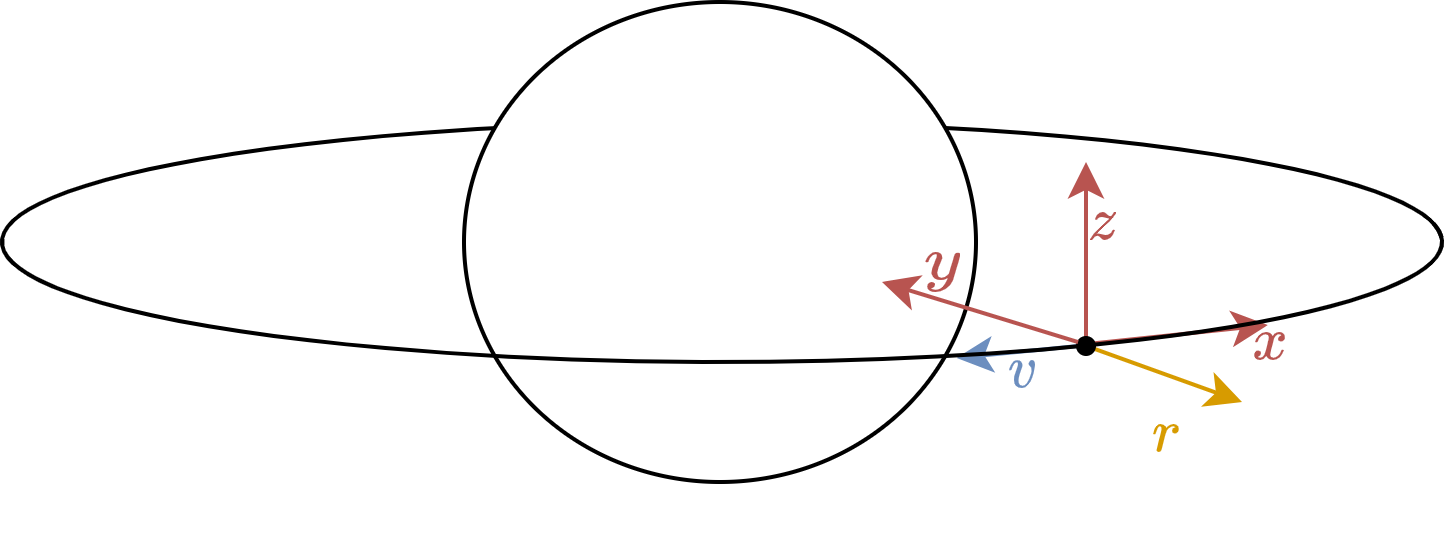
\includegraphics[width=0.9\linewidth]{assets/lvlh_frame.png}
    \caption{Local-Vertical-Local-Horizontal Frame of Reference of the Target.}
    \label{fig:lvlh_frame}
\end{figure}
If we assume the orbits of the target and the chaser to be circular, within close proximity to the target, the translational dynamics of the chaser follow the Clohessy-Wiltshire-Hill (CWH) equations (refer to Appendix \ref{app:cwh-equations}).
However, in this paper, we generalize the problem to targets that may be in elliptical orbits around the Earth.
Appendix \ref{app:ellp-undrag} describes the dynamics of relative motion in an elliptical orbit where the chaser and the target may have unequal drag constants.
These dynamics apply to the chaser with respect to the LVLH frame of reference (refer to frame L in Figure \ref{fig:target-cylinder}).
As considered in \cite{carter2002clohessy}, we assume an inverse law, $g(R)=1/R$, to model the variation in atmospheric density.
However, we realize that this inverse law does not perfectly represent the scale of the trend of atmospheric density \cite{emmert2021nrlmsis}.
As a result, we consider the corresponding ratio in variation into the drag constants $\alpha$ and $\beta$ of the target and the chaser respectively.
Such a system considers the true anomaly $\theta$ of the orbit as the independent variable, hence giving the following dynamical equations:
\begin{align}
    \boldsymbol{r}'(\theta)&=A(\theta,\theta_0)\boldsymbol{r}(\theta)+B\boldsymbol{u}(\theta)+\boldsymbol{d}(\theta, \theta_0),\label{eqn:dynamics}
\end{align}
where
\begin{subequations}
\begin{align}
    \boldsymbol{r}(\theta)&=\begin{bmatrix}
    x(\theta),y(\theta),z(\theta),x'(\theta),y'(\theta),z'(\theta)
    \end{bmatrix}^T,\\
    \boldsymbol{u}(\theta)&=\begin{bmatrix}
    u_x(\theta),u_y(\theta),u_z(\theta)
    \end{bmatrix}^T.
\end{align}
\end{subequations}
We will consider true anomaly to be the primary independent variable throughout this paper so it will be omitted as the state and input variables argument for clarity.
The relation between the true anomaly of the target and the time lapsed $t=t_{\text{curr}}-t_p$ since periapsis (the point in the path of the chaser-target system at which it is nearest to the Earth) is given as:
\begin{subequations}
\begin{align}
    M&=M_0+2\pi\frac{t}{T},\\
    M&=E-{\mathsf{e}}\sin(E),\\
    \theta&=E+2\arctan\left(\frac{\beta\sin(E)}{1-\beta\cos(E)}\right),
\end{align}
\end{subequations}
where
\begin{equation}
    \beta=\frac{{\mathsf{e}}}{1+\sqrt{1-{\mathsf{e}}^2}},
\end{equation}
$M$ is the mean anomaly of the target, $E$ is the eccentric anomaly of the target, and ${\mathsf{e}}$ is the eccentricity of the orbit of the target.
Hence, the true anomaly of the orbit can be numerically computed from time and time can be analytically computed from true anomaly.
\begin{figure}[htb]
    \centering
    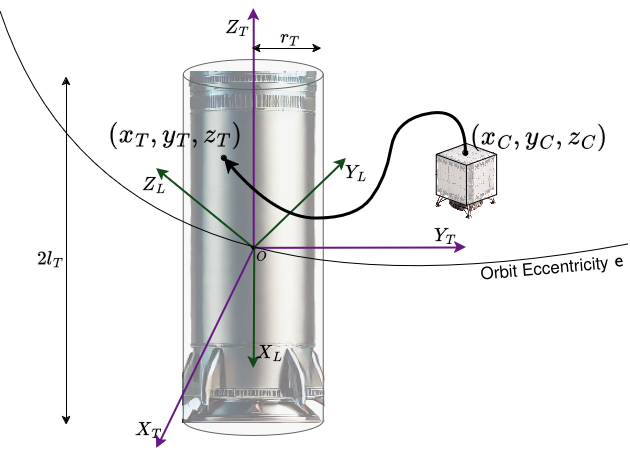
\includegraphics[width=0.85\linewidth]{assets/target-cylinder.png}
    \caption{Frames of Reference centered at the Target. The axes with subscript $T$ belong to the body frame of the target that rotates with the target and the axes with subscript $L$ belong to the local-vertical-local-horizontal (LVLH) frame that is defined in Chapter \ref{sec:relevant-knowledge}.}
    \label{fig:target-cylinder}
\end{figure}

% To follow consistent nomenclature, we use \theta in this paper to represent the true anomaly of the chaser-target system and \boldsymbol{\theta}\boldsymbol{\theta} to represent the angular position of the target.\\
\section{Summary}
This chapter presents information relevant to the setup of the problem statement.
This involves the orbital dynamics of the chaser in the frame of reference that is under consideration - the local-vertical-local-horizontal (LVLH) frame of reference.
While the Clohessy-Wiltshire-Hill equations (with time as the independent variable) are used in a circular orbit, we propose the use of the Tshauner-Henkel equations that are subsequently modified to incorporate atmospheric drag. 
These equations define the dynamics of the chaser in an elliptical orbit and use the true anomaly of the orbit as the independent variable.
As a result, the chapter also provides insight into the relation between time since periapsis and the true anomaly of the orbit through the mean anomaly and the eccentric anomaly.
\chapter{Adaptive Model Predictive Control for Trajectory Planning} \label{sec:chaser_ampc}
Rendezvous deals with the approach of the chaser from a farther location to a location close to the target.
Due to the uncertainty of orbital dynamics as a result of factors such as the elliptical nature of the orbit, electromagnetic fluctuations, atmospheric drag, and solar radiation, we propose the application of adaptive model predictive control to plan the trajectory of the chaser for rendezvous with the target.
While it is a common assumption to consider a circular orbit, this introduces an error in the dynamics of the chaser.
This further causes uncertainty even when the orbit is considered to be elliptical with an incorrect value for its eccentricity.
The dynamics of the chaser in such an orbit can be modeled using the Tshauner-Hempel equations \cite{yamanaka2002new,sinclair2015geometric}.
We also consider the effect of non-conservative forces such as quadratic atmospheric drag \cite{carter2002clohessy} on the target and the chaser which can be represented using the drag constants of the spacecraft.
We propose formulating these quantities as unknown parameters in the problem that can be learned over time based on the error in the estimated state of the chaser, $\hat{\boldsymbol{r}}$, with respect to its actual state, $\boldsymbol{r}$.
For this purpose, the chaser implements adaptive model predictive control (AMPC) wherein it plans trajectories and updates the calculated trajectory at regular intervals while also updating the estimates for the unknown quantities.

\section{Trajectory Planning} \label{ssec:rendezvous-traj-planning}
The rendezvous trajectory planning problem involves generating trajectories such that the goal state is on a sphere around the target, i.e., at a fixed predetermined distance from the target.
While the minimum possible goal radius is defined by the size and shape of the target (ref. Section \ref{sec:rendezvous-collision-constraints}), multiple intermediate spheres may be used for better observation and inertial estimation of the target.
Hence, the trajectory planning problem for rendezvous can be formulated as the following optimization problem:
\begin{align}
    \min_{\boldsymbol{r}, \boldsymbol{u}}\ J(\boldsymbol{r},\boldsymbol{u})&=h(\boldsymbol{r}(\theta_f))+\int_{\theta_0}^{\theta_f} \left((\boldsymbol{r}-\boldsymbol{r}_f)^TQ(\boldsymbol{r}-\boldsymbol{r}_f)+\boldsymbol{u}^TR\boldsymbol{u}\right)d\theta
\end{align}
\addtocounter{equation}{-1}
\vspace{-4ex}
\begin{subequations}
\begin{align}
    \textrm{s.t. } & \boldsymbol{r}'=A(\theta)\boldsymbol{r}+B\boldsymbol{u}+\boldsymbol{d}(\theta),\hspace{8em}\\
    & \boldsymbol{r}(\theta_0)=\boldsymbol{r}_0,\quad\boldsymbol{r}\in{\mathcal{C}}_R,\label{eqn:radial-limit-constraint}\\
    & \boldsymbol{v}\in{\mathcal{V}},\quad\boldsymbol{u}\in{\mathcal{U}},
\end{align}
\end{subequations}
where $\boldsymbol{r}^T=\left[\boldsymbol{p}^{T},\ \boldsymbol{v}^{T}\right]$ is the state of the system consisting of its position $\boldsymbol{p}$ and velocity $\boldsymbol{v}$ such that the system dynamics are given by the extended Tshauner-Hempel equations (explained in Appendix \ref{app:ellp-undrag}), $\boldsymbol{r}_0$ represents the starting point of the chaser, final state cost function $h(\boldsymbol{r}(\theta_f))$ is minimized to move closer to the target, and ${\mathcal{V}}$ and ${\mathcal{U}}$ represents the set of permissible velocities and control inputs of the chaser.
The additional non-convex radial-limit constraint in Equation \ref{eqn:radial-limit-constraint} ensures that the chaser remains outside all possible locations of the target, hence avoiding collisions.
As a result, the set of feasible locations is defined as ${\mathcal{C}}_R$.
This is described in detail in Section \ref{sec:rendezvous-collision-constraints}.

Docking is the final process of attaching the chaser to the target after the chaser has reached close proximity.
This is identical in structure and dynamics to rendezvous.
However, in order to make physical contact feasible, the collision constraints are modified with consideration of the physical (such as the angular velocity) and inertial (such as the moment of inertia) parameters of the target.
As a result, the radial-limit constraint is replaced by a target-limit constraint $\boldsymbol{r}(\theta)\in{\mathcal{C}}_D$ such that the chaser does not collide with the target.
Moreover, the final state cost function is made stricter to achieve docking with the target.
Additionally, to prevent plume impingement, the permissible control input set ${\mathcal{U}}$ can be made stricter \cite{starek2017fast}.
We do not consider this in this paper but propose using this approach in practice.

\section{Rendezvous and Docking Constraints} \label{sec:constraints}
\subsection{Time-Varying Final State Constraint}
\label{sec:time-varying-final-state-constraint}
Although the docking position is fixed relative to the target, it is rotating in the LVLH frame.
As a result, we incorporate a time-varying final state heuristic $\zeta(\boldsymbol{r}(\theta_f))$ such that the chaser tracks and attaches to the target at a set docking point.
The upper bound of this heuristic is decreased sequentially in the rendezvous operation to emulate observation spheres.
On the other hand, to facilitate docking, this heuristic is set to zero for docking.
Let the desired docking point be represented as $\left.\boldsymbol{\rho}_{\theta_f,T}\right|_{\theta_T=0}$ for when the target is at no rotation.
The final state heuristic can be defined using the Newton-Euler equations as follows:
\begin{align}
    \boldsymbol{\theta}_T(\theta)&=\begin{bmatrix}\alpha_T(\theta)&\beta_T(\theta)&\gamma_T(\theta)\end{bmatrix},\\
    \dot{\boldsymbol{\theta}}_T(t)&=\boldsymbol{\omega}_T(t),\\
    I\dot{\boldsymbol{\omega}}_T(t)&=-\boldsymbol{\omega}_T(t)\times I\boldsymbol{\omega}_T(t) + \boldsymbol{\tau}_T(t),\\
    \zeta(\boldsymbol{r}(\theta_f))&=\boldsymbol{r}(\theta_f)-\left.R(\theta_f)\boldsymbol{\rho}_{\theta_f}\right|_{\theta_T=0},
\end{align}
where $R(\theta_f)$ is the rotation matrix at the final true anomaly $\theta_f$ (we consider all angles to be described using Tait-Bryan rotations), $\boldsymbol{\tau}_T(t)=0$ until the end of docking, and time $t$ and true anomaly $\theta$ are interchangeable using the relations given in Section \ref{sec:relevant-knowledge}.

For rendezvous, we bound this final state heuristic by a positive ``radius" since it is not feasible to reach the final state while operating under the time-invariant rendezvous collision constraint (explained in Section \ref{sec:rendezvous-collision-constraints}).
This gives us the final state cost for rendezvous as follows:
\begin{equation}
    \label{eqn:rendezvous-cost}
    h(\boldsymbol{r}(\theta_f))|_{\text{rdv}}=Q_\text{rdv}\max{\left(||\zeta(\boldsymbol{p}(\theta_f))||-r_R, 0\right)}.
\end{equation}
For docking, we define the final state cost so that this heuristic approaches zero at the final true anomaly:
\begin{equation}
    h(\boldsymbol{r}(\theta_f))|_{\text{dkg}}=Q_\text{dkg}\zeta(\boldsymbol{p}(\theta_f)).
\end{equation}
\subsection{State and Input Bounds}
\label{sec:state-input-bounds}
Given the general definition for state and input bounds, \cite{brett2019dynamic}
\begin{align}
    ||P_{\boldsymbol{r}}\boldsymbol{r}+q_{\boldsymbol{r}}||&\leq C_{\boldsymbol{r}},\\
    ||P_{\boldsymbol{u}}\boldsymbol{u}+q_{\boldsymbol{u}}||&\leq C_{\boldsymbol{u}},
\end{align}
we define the following permissible state and input sets:
\begin{align}
    \boldsymbol{p}&\in{\mathcal{P}}:=\{\boldsymbol{p}\ |\ |p_i|<    \infty\},\quad\text{(no bound)}\\
    \boldsymbol{v}&\in{\mathcal{V}}:=\{\boldsymbol{v}\ |\ |v_i|\leq C_{V}\},\\
    \boldsymbol{u}&\in{\mathcal{U}}:=\{\boldsymbol{u}\ |\ |u_i  |\leq C_{U}\},
\end{align}
for each dimension $i=1,2,3$, where $C_{V}$ and $C_{U}$ are constants.
\subsection{Rendezvous Collision Constraints}
\label{sec:rendezvous-collision-constraints}
We define rendezvous to be necessarily bounded outside the positional limits of the target.
As a result, we constrain the chaser from entering a minimal sphere that completely bounds the target.
Since the sphere is a cyclically symmetrical shape in all directions, the rotation of the target does not affect its shape or size and, hence, the constraint is time-invariant, reducing computational complexity for the rendezvous problem.
Therefore, the rendezvous collision constraint can be written as $\boldsymbol{r}\in{\mathcal{C}}_R$ where:
\begin{equation}
    {\mathcal{C}}_R:=\{\boldsymbol{r}\ |\ ||\boldsymbol{p}||>\rho_T, \rho_T=\min\rho \text{ s.t. } ||\boldsymbol{p}_T||\leq\rho\ \forall\ \boldsymbol{p}_T\in\text{T}\}.
\end{equation}
That is, the chaser is constrained to remain outside a sphere of radius $\rho_T$ that minimally encloses the target which is represented by the set T that represents the set of points on the target that minimally defines the complete boundary of the target.
Alternatively, the constraint can be described by the minimum enclosing ellipsoid of the target (Refer to Appendix \ref{app:mee}) to minimize the distance between the chaser and the target prior to docking.
Although this demands some information regarding the shape and rotation of the target, it can be observed that the symmetry involved in such a constraint can be used to reduce complexity especially when dealing with multi-axis rotations.

\subsection{Time-Varying Docking Collision Constraints}
\label{sec:time-varying-collision-constraints}
The docking operation involves a tighter time-varying state constraint to prevent collisions between the chaser and the target while permitting docking to the boundary of the target.
The same rotational characteristics of the target described in Section \ref{sec:time-varying-final-state-constraint} introduce time-varying collision constraints for the chaser that can be represented as $\boldsymbol{r}(\theta)\in{\mathcal{C}}_D$.
This is motivated by the concept of exclusion from target space as proposed in \cite{park2017nonlinear}.

For instance, if the target is cylindrical with radius $r_T$ and length $2l_T$ centered at the origin as demonstrated in Figure \ref{fig:target-cylinder} and rotates such that its rotation matrix at time $t$ is given as $R(t)$, the permissible state set ${\mathcal{C}}_D$ for the chaser can be written as the following union:
\begin{align}
    {\mathcal{C}}_D&:={\mathcal{C}}_{D1}\cup{\mathcal{C}}_{D2},\label{eqn:or-function}
\end{align}
where
\begin{subequations}
\begin{align}
    {\mathcal{C}}_{D1}&:=\{\boldsymbol{r}(\theta)\ |\ f_{D1}=x_{\mathcal{R}}(\theta)^2 + y_{\mathcal{R}}(\theta)^2 - r_T^2\geq0\},\\
    {\mathcal{C}}_{D2}&:=\{\boldsymbol{r}(\theta)\ |\ f_{D2}=||z_{\mathcal{R}}(\theta)|| - l_T\geq0\},
\end{align}
\end{subequations}
such that the de-rotated state vector $r_{\mathcal{R}}(\theta)$ (i.e., the position of the chaser as viewed in a target-centered frame of reference that rotates with the target) is defined as:
\begin{align}
    \boldsymbol{r}_{\mathcal{R}}(\theta)&=\begin{bmatrix}
        x_{\mathcal{R}}(\theta)&y_{\mathcal{R}}(\theta)&z_{\mathcal{R}}(\theta)&\dot{x}_{\mathcal{R}}(\theta)&\dot{y}_{\mathcal{R}}(\theta)&\dot{z}_{\mathcal{R}}(\theta)
    \end{bmatrix}^T\notag\\
    &=\left(R^{-1}(\theta)\otimes I_2\right)\boldsymbol{r}(\theta).
\end{align}
Here, $A\otimes B$ represents the Kronecker product of the two matrices $A$ and $B$.
Also, we recall that ${R}^{-1}={R}^T$.
The above union can be implemented on a numerical solver using the following logic:
\begin{align}
    {\mathcal{C}}_D:=\{\boldsymbol{r}(\theta)\ |\ \text{sgn}(f_{D1})+\text{sgn}(f_{D2})\geq0\},
\end{align}
where $\text{sgn}(x)$ is the sign function such that
\begin{equation}
    \text{sgn}(x) = \begin{cases}
        1\ ,\ x>0\\
        0\ ,\ x=0\\
        -1\ ,\ x<0
    \end{cases}.
\end{equation}

\section{Estimation of Inertial and Angular Target Parameters}
\label{sec:target-estimation}
At any given time, the final docking position of the chaser is determined by the current angular position of the target and a predetermined point that is fixed in the body frame of the target.
The collision constraint in the docking problem also requires an accurate estimation of the inertial and angular parameters of the target.
While we do not directly address the estimation of these parameters in this paper, we encourage the reader to refer to \cite{setterfield2018inertial} on the estimation of the angular velocity and the moment of inertia of the target using polhode analysis of the angular momentum and energy of the target.
The estimation of the current state of the chaser depends on the accuracy of the dynamics of the chaser in the LVLH frame of the target as explained in Equation \ref{eqn:dynamics}.
These dynamics depend on the unknown parameters discussed earlier - the eccentricity of the orbit and the drag constant of the target.
In order to estimate these quantities, we introduce adaptive control using set membership identification (SMID).
As explained in \cite{morozov2020performance}, recursive feasibility (meaning that the problem remains feasible for all time) of the MPC operation requires that system uncertainty is monotonically non-increasing throughout adaptation.
This is achieved in our implementation of adaptive control using SMID since the feasible solution set (FSS) shrinks monotonically over time (Refer to Step 2 of Algorithm \ref{alg:smid}).
The progression of estimation using this SMID implementation is demonstrated in Figure \ref{fig:smid}.
\begin{figure}[t]
    \centering
    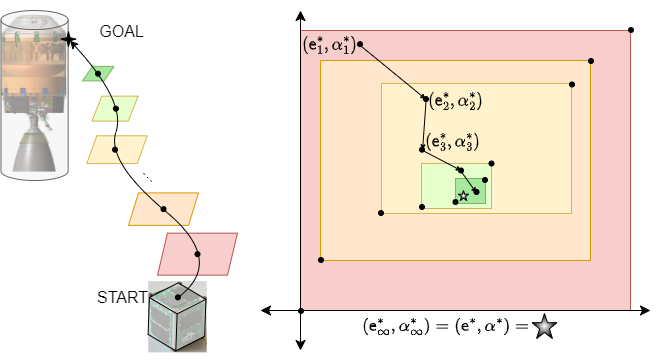
\includegraphics[width=0.95\linewidth]{assets/smid.png}
    \caption{Implementation of the Set Membership Identification (SMID) algorithm}
    \label{fig:smid}
\end{figure}
\begin{algorithm}
    \begin{algorithmic}[1]
        \small
        \Statex \textbf{Input:} $\boldsymbol{w}(\theta), \boldsymbol{u}(\theta) \text{ for } \theta\in[\theta_0,\theta_f]$, existing ${\mathcal{E}}$, ${\mathcal{A}}$; \, \textbf{Output:} updated ${\mathcal{E}}$, ${\mathcal{A}}$
        
        \State \underline{Generate a Feasible Solution Set (FSS)}
        \Statex \indent $\underline{{\mathsf{e}}}_{est} = \min{\mathsf{e}}$,
        \Statex \indent $\overline {{\mathsf{e}}}_{est} = \max{\mathsf{e}}$,
        \Statex \indent $\underline{ \alpha     }_{est} = \min{\alpha}$,
        \Statex \indent $\overline { \alpha     }_{est} = \max{\alpha}$, such that 
        \Statex \indent \indent $\boldsymbol{r}'=A(\theta; \alpha, \mathsf{e})\boldsymbol{r}+B(\theta; \alpha, \mathsf{e})\boldsymbol{u}+\boldsymbol{d}(\theta; \alpha, \mathsf{e})$,
        \Statex \indent \indent $\boldsymbol{p}(\theta_0)=\boldsymbol{w}(\theta_0)$, $||\boldsymbol{p}(\theta_f)-\boldsymbol{w}(\theta_f)||\leq D$,
        \Statex \indent \indent ${\mathsf{e}}\in{\mathcal{E}}$, $\alpha  \in{\mathcal{A}}$.
        
        \State \underline{Define the new FSS}
        \Statex \indent ${\mathcal{E}}_{new}={\mathcal{E}}\cap[\underline{{\mathsf{e}}}_{est}, \overline{{\mathsf{e}}}_{est}]$,
        \Statex \indent ${\mathcal{A}}_{new}={\mathcal{A}}\cap[\underline{\alpha}_{est},   \overline{\alpha}_{est}]$.
    
        \State \underline{Verify the new FSS}
        \Statex \indent Attempt to generate $\boldsymbol{r}(\theta)$ such that
        \Statex \indent \indent $\boldsymbol{r}'=A(\theta; \alpha, \mathsf{e})\boldsymbol{r}+B(\theta; \alpha, \mathsf{e})\boldsymbol{u}+\boldsymbol{d}(\theta; \alpha, \mathsf{e})$,
        \Statex \indent \indent $\boldsymbol{p}(\theta_0)=\boldsymbol{w}(\theta_0)$, $\boldsymbol{p}(\theta_f)\approx \boldsymbol{w}(\theta_f)$,
        \Statex \indent \indent ${\mathsf{e}}\in{\mathcal{E}}_{new}$, $\alpha  \in{\mathcal{A}}_{new}$.
    
        \State \underline{Compare and Update the FSS}
        \Statex \indent If Step 3 works:
        \Statex \indent \indent ${\mathcal{E}}\leftarrow{\mathcal{E}}_{new}$,
        \Statex \indent \indent ${\mathcal{A}}\leftarrow{\mathcal{A}}_{new}$.
        % \Statex \indent else: do nothing
        
        \State \underline{Update Data Range for Adaptation}
        \Statex \indent Consider new data by updating $\theta_0$ and $\theta_f$ as:
        \Statex \indent \indent $\Delta\theta = \theta_f - \theta_0$,
        \Statex \indent \indent $\theta_0 \leftarrow \theta_f$,
        \Statex \indent \indent $\theta_f \leftarrow \theta_f + \Delta \theta$.
    \end{algorithmic}
    \caption{A single iteration of \textbf{set membership identification (SMID)}}
    \label{alg:smid}
\end{algorithm}
We draw motivation from the idea of MSAC-MPC in \cite{tang2023indirect} to stop adaptation after a fixed number of iterations for computational simplicity.
We choose to stop adaptation at the end of rendezvous (before the start of docking) based on the shrunken size of the uncertainty tube.
The time or number of iterations for adaptation can be picked based on the accuracy of estimation.

We also assume that the intervals considered for the parameters are convex such that every value within two boundary values satisfies convex conditions.
This need not hold true when the intervals are large due to the nonlinear nature of the state space.
As a result, we recommend splitting the intervals such that each sub-interval is convex and treating the new FSS estimate as the union of all feasible sub-intervals.

\section{Summary}
This chapter focuses on the problem of chaser trajectory optimization to conduct rendezvous and docking to a point on the target.
A feasible trajectory is generated with cost minimization of the control effort and error from the final state while satisfying the relative motion dynamics of the chaser satellite in close proximity to the target in orbit.
This is followed by a discussion of the implementation of the set membership identification (SMID) algorithm to estimate the eccentricity of the orbit and the drag constant of the target.
The chapter also provides insight into the final state constraint that varies with time owing to the rotation of the target.
This involves convergence onto a rendezvous sphere followed by docking onto a predetermined point on the target.
This is followed by a discussion on the bounds of the states and the control inputs of the chaser.
The chapter ends by discussing the collision constraints associated with rendezvous and docking of which the latter is time-varying due to the rotation of the target.
\chapter{Incorporation of Dynamic Tubes for Constraint Satisfaction and Extension to Multiple Agents}
\label{sec:dynamic-tube}
Following the determination of the docking point of the chaser, the chaser plans a trajectory from the current position to the calculated goal position on the target.
As a result of SMID-based adaptive control, the chaser has significantly improved estimates of uncertain parameters (eccentricity and drag constant) by the completion of rendezvous and it is capable of planning a trajectory from a start position to a docking point on the target.
However, while the docking point is on the surface of the target, the target also behaves as an obstacle in the trajectory planning problem of the chaser.
The resulting high degree of proximity from physical contact required for docking increases the likelihood of a chaser-target collision.
While the time-varying docking constraint (Section \ref{sec:time-varying-collision-constraints}) prevents the nominal state from such a collision, the inaccuracy in estimated parameters may lead to a violation of this constraint.

In order to avoid such constraint violations, we use dynamic robust control-invariant (RCI) tubes as proposed in \cite{brett2019dynamic} to constrain the possible error in the chaser state, hence using adaptive dynamic tube MPC (ADTMPC) for chaser trajectory planning.
As a result, the general nominal trajectory planning problem can be formulated as the following optimization problem:
\begin{align}
    \min_{\hat{\boldsymbol{u}}}\ J(\hat{\boldsymbol{r}},\hat{\boldsymbol{u}})&=h(\hat{\boldsymbol{r}}(\theta_f))+\int_{\theta_0}^{\theta_f} \left((\hat{\boldsymbol{r}}-\boldsymbol{r}_f)^TQ(\hat{\boldsymbol{r}}-\boldsymbol{r}_f)+\hat{\boldsymbol{u}}^TR\hat{\boldsymbol{u}}\right)d\theta\label{eqn:dynamic-tubes-equation}
\end{align}
\addtocounter{equation}{-1}
\vspace{-4ex}
\begin{subequations}
\begin{align}
    \textrm{s.t. } & \hat{\boldsymbol{r}}'=A(\theta)\hat{\boldsymbol{r}}+B(\theta)\hat{\boldsymbol{u}}+\hat{\boldsymbol{d}}(\theta), \ \ \hat{\boldsymbol{u}}\in\hat{\mathcal{U}},\\
    & \hat{\boldsymbol{r}}(\theta_0)=\boldsymbol{r}(\theta_0)=\boldsymbol{r}_0,\quad\hat{\boldsymbol{r}}\in\hat{{\mathcal{C}}},\\
    & \boldsymbol{\phi}'=-\hat{\boldsymbol{\alpha}}\boldsymbol{\phi}+\boldsymbol{\Delta}(\hat{\boldsymbol{r}})+\boldsymbol{D}+\boldsymbol{\eta},\ \ \boldsymbol{\phi}(\theta_0)=\boldsymbol{\phi}_0,\\
    & \boldsymbol{\Omega}'=A_\lambda\boldsymbol{\Omega}+B_\lambda\boldsymbol{\phi},\quad\boldsymbol{\Omega}(\theta_0)=|\Tilde{\boldsymbol{r}}_0|,
\end{align}
\end{subequations}
where $A_\lambda=\text{diag}(\boldsymbol{\lambda})=\text{diag}([\lambda_1,~\lambda_2,~\lambda_3])$, $B_\lambda=I_{3}$, and $h(\cdot)$ and $\hat{{\mathcal{C}}}$ are determined based on the operation, e.g., rendezvous or docking.
Here, $\phi(\theta)$ represents the boundary layer of the tube and $\Omega(\theta)$ represents the tube geometry.
Also, $\hat{{\mathcal{C}}}$ refers to the tightened set of constraints discussed in detail in Sections \ref{sec:bound-shrinking} and \ref{sec:non-convex_const_expansion}.
\begin{figure}[htb]
    \centering
    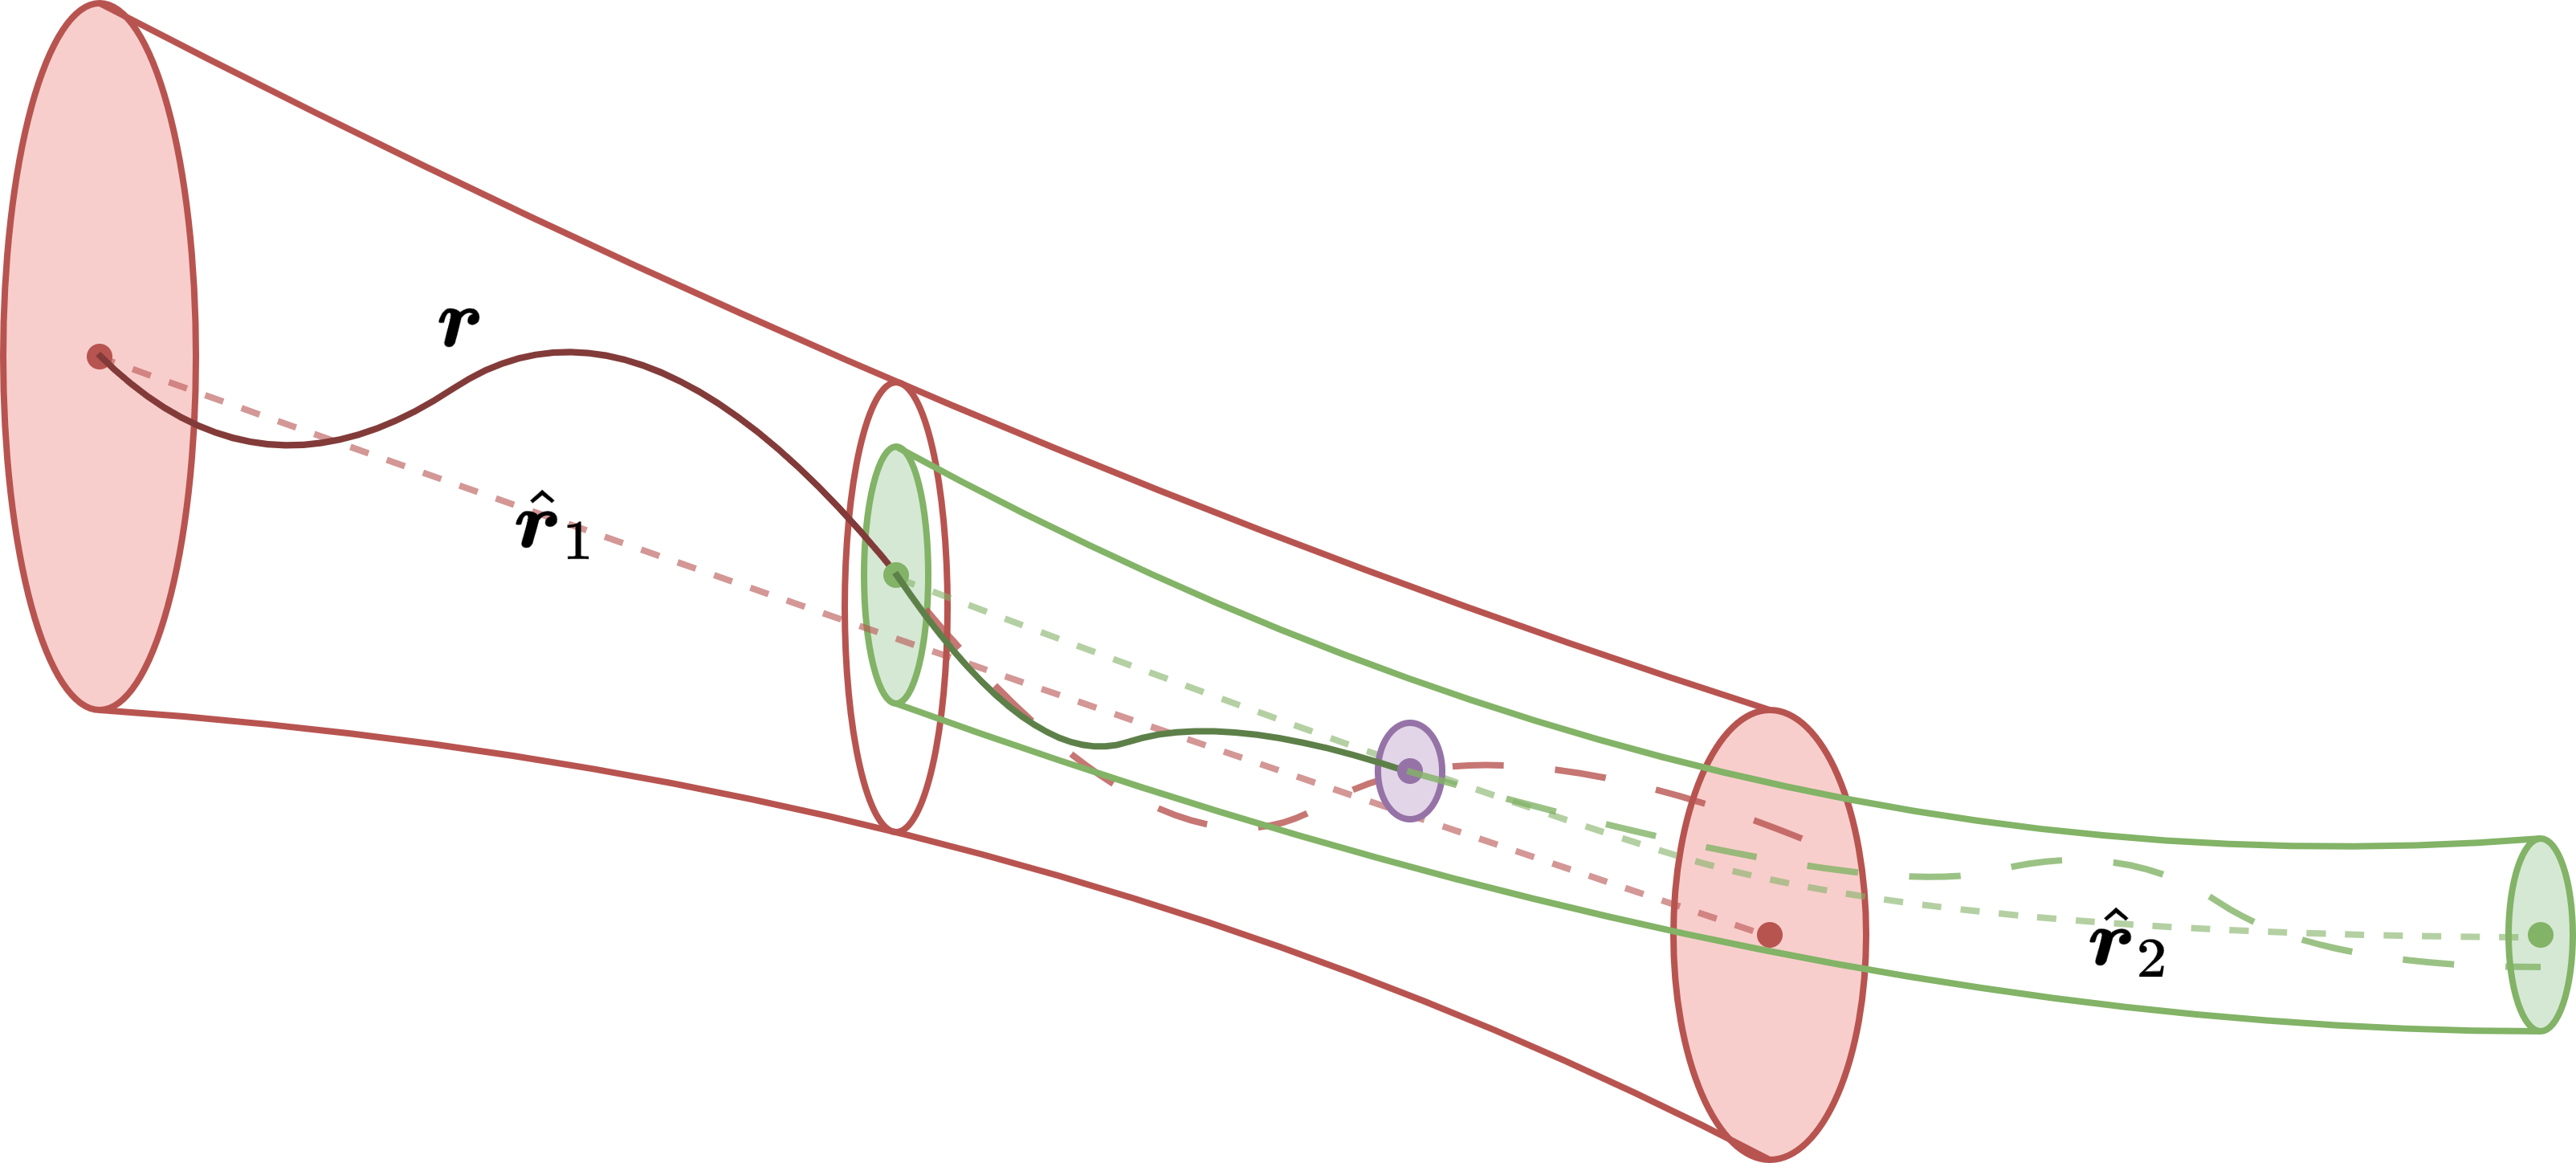
\includegraphics[width = 0.96\linewidth]{assets/adtmpc.png}
    \caption{Adaptive Tube Model Predictive Control. The tubes represent the permissible region for the actual trajectory of the chaser. The dotted lines represent the nominal states and the dashed lines represent the actual states. Due to the receding horizon nature of the problem, the spacecraft plans a new trajectory before the final state is reached.}
    \label{fig:adtmpc}
\end{figure}
\section{Ancillary Controller and the Actual Control Input}
The boundary-layer sliding mode controller (BLSC) that supports the robust tube mechanism is introduced as an ancillary controller to the nominal input that is obtained from the trajectory planning problem.
Hence, the actual control input $\boldsymbol{u}$ can be written as the sum of the nominal input $\hat{\boldsymbol{u}}$ and this ancillary controller $\Tilde{\boldsymbol{u}}$:
\begin{alignat}{2}
    \boldsymbol{u}&=\hat{\boldsymbol{u}}+\Tilde{\boldsymbol{u}},\\
    \Tilde{\boldsymbol{u}}&=B(\boldsymbol{r})^{-1}\left(A^V\Tilde{\boldsymbol{r}}-A_\lambda\Tilde{\boldsymbol{v}}-\text{sat}\left(\frac{\boldsymbol{s}}{\boldsymbol{\phi}}\right)[K(\boldsymbol{r})]\right),
\end{alignat}
where the sliding variable $\boldsymbol{s}$ is defined as:
\begin{alignat}{2}
    \boldsymbol{s}=\Tilde{v}+A_\lambda\Tilde{p},
\end{alignat}    
and $[K(\boldsymbol{r})]=\text{diag}(K(\boldsymbol{r}))$ can be calculated as:
\begin{subequations}
\begin{alignat}{2}
    \boldsymbol{\phi}'&=-\boldsymbol{\alpha}\boldsymbol{\phi}+\boldsymbol{\Delta}(\boldsymbol{r})+\boldsymbol{D}+\boldsymbol{\eta},\\
    K(\boldsymbol{r})&=\boldsymbol{\Delta}(\boldsymbol{r})+\boldsymbol{D}+\boldsymbol{\eta}-\phi'\\
    &=(\boldsymbol{\Delta}(\boldsymbol{r})-\boldsymbol{\Delta}(\hat{\boldsymbol{r}}))+\boldsymbol{\alpha}\boldsymbol{\phi}\\
    &=\boldsymbol{\Delta}(\Tilde{\boldsymbol{r}})+\boldsymbol{\alpha}\boldsymbol{\phi}.\label{eqn:K(r)}
\end{alignat}
\end{subequations}
Here, $\boldsymbol{\Delta}(\boldsymbol{r})$ is the maximum bound on the dynamics $\boldsymbol{f}=\hat{\boldsymbol{f}}+\Tilde{\boldsymbol{f}}$ where $\hat{\boldsymbol{f}}$ is the nominal dynamics and $\Tilde{\boldsymbol{f}}$ is the bounded model error such that $|\Tilde{\boldsymbol{f}}|\leq\boldsymbol{\Delta}(\boldsymbol{r})$.
Also, $\boldsymbol{D}$ is the maximum bound on the disturbance $\boldsymbol{d}(\theta)$ in the dynamics such that $\boldsymbol{d}(\theta)\leq\boldsymbol{D}$, and $\boldsymbol{\eta}$ is a predefined quantity.
\section{Shrinking of State and Input Bounds}
\label{sec:bound-shrinking}
State and input constraints need to be modified due to the non-zero tracking error $\Tilde{\boldsymbol{r}}(\theta)$.
The state and input bounds defined in Section \ref{sec:state-input-bounds} must be modified to account for the non-zero tracking error and control input error.
We incorporate the tightening equations proposed in \cite{brett2019dynamic} into the optimization problem in Equation \ref{eqn:dynamic-tubes-equation} as a modified set of constraints $\hat{\boldsymbol{r}}\in\hat{{\mathcal{C}}}$ that can be expanded as follows:
\begin{align}
    ||P_{\hat{\boldsymbol{r}}}\hat{\boldsymbol{r}}(\theta)+q_{\hat{\boldsymbol{r}}}||&\leq C_{\hat{\boldsymbol{r}}}-||P_{\hat{\boldsymbol{r}}}\Tilde{\boldsymbol{r}}(\theta)||,\\
    ||P_{\hat{\boldsymbol{u}}}\overline{B}^{-1}\hat{\boldsymbol{u}}(\theta)+q_{\hat{\boldsymbol{u}}}||&\leq C_{\hat{\boldsymbol{u}}}-||P_{\hat{\boldsymbol{u}}}\overline{B}^{-1}\Tilde{\boldsymbol{u}}_{fb}||.
\end{align}
Hence, we may rewrite the state and input bounds as:
\begin{align}
    \hat{\boldsymbol{p}}&\in{\mathcal{P}}:=\{\hat{\boldsymbol{p}}\ |\ |\hat{p}_i|<    \infty\},\quad\text{(no bound)}\\
    \hat{\boldsymbol{v}}&\in{\mathcal{V}}:=\{\hat{\boldsymbol{v}}\ |\ |\hat{v}_i|\leq C_{V}-|\Tilde{v}|\},\\
    \hat{\boldsymbol{u}}&\in{\mathcal{U}}:=\{\hat{\boldsymbol{u}}\ |\ |\hat{u}_i  |\leq C_{U}-|\Tilde{u}_{fb,i}|\},
\end{align}
where $i=1,2,3$ and
\begin{subequations}
\begin{alignat}{2}
    \Tilde{\boldsymbol{u}}_{fb}&=\left|\overline{F}+A_{\lambda}\Tilde{\boldsymbol{r}}\right.&&\left.+\overline{K}\right|,\\
    \overline{F}&=A^V\overline{\boldsymbol{r}},&&\underline{F}=A^V\underline{\boldsymbol{r}},\\
    \overline{K}&=K\left(\overline{\boldsymbol{r}}\right),&&\underline{K}=K\left(\underline{\boldsymbol{r}}\right),\\
    \overline{\boldsymbol{r}}&=\hat{\boldsymbol{r}}+|\Tilde{\boldsymbol{r}}|,&&\underline{\boldsymbol{r}}=\hat{\boldsymbol{r}}-|\Tilde{\boldsymbol{r}}|,
\end{alignat}
\end{subequations}
where $K(\cdot)$ is defined in Equation \ref{eqn:K(r)}.
\section{Expansion of Non-Convex State Constraints}
\label{sec:non-convex_const_expansion}
We realize that, although the inputs are bound in a convex space, the state space is non-convex either due to the radial-limit constraint (Equation \ref{eqn:radial-limit-constraint}) during rendezvous or due to the target-limit constraint (Section \ref{sec:time-varying-collision-constraints}) during docking.
These constraints need to be expanded resembling how the convex bounds are shrunk in Section \ref{sec:bound-shrinking}.
As a result, the radial-limit constraint can now be rewritten as $\hat{\boldsymbol{r}}\in\hat{{\mathcal{C}}}_R$ where:
\begin{alignat}{2}
    \hat{{\mathcal{C}}}_R:=\{\hat{\boldsymbol{r}}\ |\ ||\hat{\boldsymbol{p}}||>\rho_T+||\Tilde{\boldsymbol{p}}||, \rho_T=\min\rho \text{ s.t. } ||\boldsymbol{p}_T||\leq\rho\ \forall\ \boldsymbol{p}_T\in\text{T}\}.
\end{alignat}
Similarly, the chaser-target collision avoidance constraint for docking must be expanded such that the dynamic RCI tube can at most touch the target.
Since distances are invariant to rotations, the expansion of the constraint is not affected by the rotation of the position of the chaser with respect to the target.
As a result, the constraint in Equation \ref{eqn:or-function} can be rewritten as:
\begin{align}
    \hat{{\mathcal{C}}}_D&:=\hat{{\mathcal{C}}}_{D1}\cup\hat{{\mathcal{C}}}_{D2},\label{eqn:expanded-target-limit-constraint}
\end{align}
where
\begin{subequations}
\begin{align}
    \hat{{\mathcal{C}}}_{D1}&:=\{\boldsymbol{r}(\theta)\ |\ f_{D1}\geq0\},\\
    \hat{{\mathcal{C}}}_{D2}&:=\{\boldsymbol{r}(\theta)\ |\ f_{D2}\geq0\}.
\end{align}
\end{subequations}
Here, the constraint functions $f_{D1}$ and $f_{D2}$ are defined as:
\begin{subequations}
\begin{align}
    f_{D1}&=x_{\mathcal{R}}(\theta)^2 + y_{\mathcal{R}}(\theta)^2 - (r_T+||\Tilde{\boldsymbol{p}}||)^2,\\
    f_{D2}&=||z_{\mathcal{R}}(\theta)|| - (l_T+||\Tilde{\boldsymbol{p}}||),
\end{align}
\end{subequations}
We realize that this can be slightly conservative on the edges of the target.
This can be rectified by adding a third constraint while ignoring the existing two constraints at the edge to provide a rounded cylinder constraint.
Similarly, it can be made less conservative by constraining each dimension separately, giving:
\begin{subequations}
\begin{align}
    f_{D1}&=x_{\mathcal{R}}(\theta)^2 + y_{\mathcal{R}}(\theta)^2 - \left(r_T+\left|\left|\begin{bmatrix}
        \Tilde{x}_{\mathcal{R}}&\Tilde{y}_{\mathcal{R}}
    \end{bmatrix}\right|\right|\right)^2,\\
    f_{D2}&=||z_{\mathcal{R}}(\theta)|| - (l_T+||\Tilde{z}_{\mathcal{R}}||),
\end{align}
\end{subequations}
where, for $r_i\in[x,y,z]$,
\begin{align}
    \Tilde{r}_{i, {\mathcal{R}}}=r_{i, {\mathcal{R}}}(\theta)-\hat{r}_{i, {\mathcal{R}}}(\theta).
\end{align}

\section{Extension to Multi-Chaser Systems}
\label{sec:multi-agent}
Although several uncontrollable objects in orbit are relatively small, some of the most concerning ones (with respect to the risk they pose to vital controllable systems) are large rocket bodies \cite{mcknight2021identifying}.
A single chaser that may be as large as a conventional satellite may not be capable of providing sufficient thrust or leverage to detumble such an object.
As a result, we propose the use of multiple chasers to simultaneously act on the target for tumble minimization and deorbiting.
In the process of rendezvous and docking, such a multi-agent system will require additional constraints to prevent collisions between themselves.
Moreover, for space debris that is much larger than the chaser, the docking of the chaser to the target decreases the degrees of freedom of the system due to thrusters in the direction of the target.
This implies the need for multiple chasers in the scenario of multi-axis rotations and operations that follow detumbling such as deorbiting the target by directing it into a graveyard orbit.

The separate implementation of the rendezvous and docking problem proposed in Section \ref{sec:chaser_ampc} for each chaser in a multi-agent context introduces the risk of collisions between chasers and the possibility of multiple chasers picking the same docking point.
For the multi-agent problem, the sequential implementation of goal determination and allocation from a set of possible goal states followed by individual trajectory planning may be different in solution and hence in optimality from the combined problem of distributed optimal control.
The first approach does not take into account the positions of other agents when planning individual trajectories, which could lead to collisions.
As a result, we suggest the use of the combined problem of distributed optimal control where the same problem is solved by each chaser based on the initial state of all chasers and a common final state manifold.
Moreover, the problem requires focusing on minimizing the total cost of the operation instead of the individual costs of each chaser.
On the other hand, this brings up the possibility of resource depletion for individual chasers due to which the total control input for each chaser over time needs to be constrained.
As a result, the multi-agent problem for rendezvous can be written as follows:
\begin{align}
    \min_{\boldsymbol{u}}\ \ J(\boldsymbol{r},\boldsymbol{u})=\sum_{i=1}^{N_C}\int_{\theta_0}^{\theta_f}\left(\boldsymbol{r}_i^TQ_i\boldsymbol{r}_i+\boldsymbol{u}_i^TR_i\boldsymbol{u}_i\right)d\theta
\end{align}
\addtocounter{equation}{-1}
\vspace{-4ex}
\begin{subequations}
\begin{align}
    \textrm{s.t. } & \boldsymbol{r}_i'=A(\theta)\boldsymbol{r}_i+B(\theta)\boldsymbol{u}_i+\boldsymbol{d}(\theta),\\
    & \boldsymbol{r}_i(\theta_0)={\boldsymbol{r}}_{i,0},\quad h(\boldsymbol{r}_i(\theta_f))=0,\\
    & \boldsymbol{r}(\theta)\in{\mathcal{C}}_{i,T}\cap{\mathcal{C}}_{i,j},\quad\boldsymbol{u}_i\in{\mathcal{U}}_i,\label{eqn:multi-agent-rendezvous}
\end{align}
\end{subequations}
where $i,j\in[1,2,\ldots,N_C]$ and $j>i$.
Here, while the chaser-target collision constraints, ${\mathcal{C}}_{i,T}$, can be expanded as explained in Section \ref{sec:time-varying-collision-constraints}, the inter-chaser collision constraints can be written as follows:
\begin{align}
    {\mathcal{C}}_{i,j}&=\{\boldsymbol{r}_i(\theta):||\boldsymbol{r}^P_{i}-\boldsymbol{r}^P_{j}||-\epsilon_{i,j}\},
\end{align}
where $\epsilon_{i,j}$ is predetermined based on the geometry of chasers $i$ and $j$. We replace the final state cost function with an equivalent final state constraint $h(\boldsymbol{r}_i(\theta_f))=0$ such that:
\begin{align}
    h(\boldsymbol{r}_i(\theta_f))&=\inf_{\rho\in{\mathcal{T}}_{\text{dock}}}\left(||\boldsymbol{r}_i(\theta_f)-\rho||\right),
\end{align}
where ${\mathcal{T}}_{\text{dock}}$ represents the set of docking points on the target.
A similar multi-agent problem can be written for the docking problem by replacing the chaser-target collision constraint accordingly.

\section{Summary}
This chapter proposes the use of dynamic tubes to introduce robustness to the chaser trajectory planning problem.
This subsequently leads to the modification of the control input of the chaser.
The bounds on the convex constraints of the modified nominal system are shrunk to avoid infeasibility and, equivalently, the concave constraints are expanded to prevent collisions.
Following this, the chapter discusses the extension of the proposed single-chaser rendezvous and docking problem to a multi-chaser scenario.
It highlights the challenges and proposes a distributed optimal control approach for solving the problem.
Such a multi-agent rendezvous and docking problem requires additional constraints to prevent collisions between chasers.
The chapter also briefly discusses the selection of docking points given multiple agents.
\chapter{Target Deflection}
\label{sec:target-deflection}
Once the chaser has docked with the target at some position $\boldsymbol{d}$ with respect to the center of the target, any force $\boldsymbol{f}$ applied by the chaser thrusters translates to a torque $\boldsymbol{\tau}$ applied on the target as:
\begin{align}
    \boldsymbol{\tau} = \boldsymbol{d}\times\boldsymbol{f}.
\end{align}
In the multi-agent scenario (with $N_C$ chasers), the net torque acting on the target can be written as:
\begin{align}
    \boldsymbol{\tau} = \sum_{i=1}^{N_C}\boldsymbol{d}_{i}\times\boldsymbol{f}_{i}.
\end{align}
As a result, the dynamics of the target can be written using the Newton-Euler equations as follows:
\begin{align}
    \dot{\boldsymbol{\theta}}(t)&=\boldsymbol{\omega}(t),\\
    I\dot{\boldsymbol{\omega}}(t)&=-\boldsymbol{\omega}(t)\times I\boldsymbol{\omega}(t)+\sum_{i=1}^{N_C}\boldsymbol{d}_{i}\times\boldsymbol{f}_{i}.
\label{eqn:newton-euler-target-detumbling}
\end{align}
We draw motivation from \cite{liu2014in} in stating that the chaser-target system behaves as a compound satellite.
As a result, the total moment of inertia of the system is determined by that of the target and that of the chaser and the position of the chaser with respect to the center of mass of the target.
For simplicity, we will assume that this net moment of inertia is known.
On the other hand, it is possible to calculate the net moment of inertia using the parallel axis theorem.

This chapter focuses on calculating the optimal docking position and control input trajectory of the chaser(s) such that the final angular velocity of the target is zero while minimizing a cost function proportional to the net control input.
The interaction of multiple chasers with the target is more complicated than the single-agent case since one agent interacting with the object could change the environment for all other agents.
To simplify this issue, for the multi-agent scenario, we propose the simultaneous attachment of all chasers and the application of thrust so as to stop tumble only after all chasers have been attached to the target.\\
Since the Newton-Euler equations are in the time domain, in this chapter, we retreat to the traditional form of representing, differentiating, and integrating variables with respect to time (note that the same operations have been performed with respect to true anomaly in previous chapters).

\section{Calculation of Docking Points and Force Application}
In order to calculate the docking points for each chaser $i\in[1,2,\ldots,N_C]$, we minimize the sum of the integral of forces applied by each chaser. This optimal control problem is governed by the Newton-Euler equations described above in Equation \ref{eqn:newton-euler-target-detumbling}. The moment of inertia and the initial angular velocity of the target are obtained from techniques such as polhode analysis as explained in Section \ref{sec:target-estimation}. Since the problem aims to stop the tumble of the target, the final angular velocity of the target is set to zero. Accounting for these constraints, the detumbling problem can be expressed as the following dynamic optimization problem:
\begin{align}
    \min_{\boldsymbol{d}_{i},\boldsymbol{f}_{i}}\ &J\left(\boldsymbol{f}_{i}(t),\boldsymbol{d}_{i},\boldsymbol{\theta}_T(t), \boldsymbol{\omega}_T(t)\right) =\int_{t_0}^{t_f}\sum_{i=1}^N||\boldsymbol{f}_{i}(t)||^2dt
\end{align}
\addtocounter{equation}{-1}
\vspace{-4ex}
\begin{subequations}
\begin{align}
    \textrm{s.t. } & \dot{\boldsymbol{\theta}}(t)=\boldsymbol{\omega}(t),\\
    & I\dot{\boldsymbol{\omega}}(t)=-\boldsymbol{\omega}(t)\times I\boldsymbol{\omega}(t)+\sum_{i=1}^{N_C}\boldsymbol{d}_{i}\times\boldsymbol{f}_{i},\\
    & \boldsymbol{\omega}(t_0)=\boldsymbol{\omega}_0,\quad\boldsymbol{\omega}(t_f)=0,\\
    & \boldsymbol{f}_{i}\in{\mathcal{F}}_i,\\
    & \boldsymbol{d}_C\in{\mathcal{G}}_T. \label{eqn:geometrical-constraint}
\end{align}
\end{subequations}
Here, ${\mathcal{F}}_i$ represents the input bounds on chaser $i$ and ${\mathcal{G}}_T$ represents the geometrical constraint of the target on the docking point of the chaser. For example, if the target is a cylinder of radius $r_T$ and length $2l_T$ centered at the origin (assuming docking on the curved surface), the geometrical constraint in Equation \ref{eqn:geometrical-constraint} can be expanded as:
\begin{align}
    {\mathcal{G}}_T:={\mathcal{G}}_{T1}\cap{\mathcal{G}}_{T2},
\end{align}
where
\begin{subequations}
\begin{align}
    {\mathcal{G}}_{T1}&:=\{\boldsymbol{d}_C\ |\ \boldsymbol{d}_{C,x}^2+\boldsymbol{d}_{C,y}^2=r_T^2\},\\
    {\mathcal{G}}_{T2}&:=\{\boldsymbol{d}_C\ |\ |\boldsymbol{d}_{C,z}|<l_T\}.
\end{align}
\end{subequations}
For the problem of calculating docking points, we ignore the rotation of the target. Instead, this rotation is considered in the formulation of the final state constraint for the docking trajectory problem as shown in Section \ref{sec:time-varying-final-state-constraint}.
\section{Discretization of Docking Points}
Due to the likelihood that specific points on the target (such as existing docking ports) will support docking better than others, we propose extending the above problem such that the docking position $\boldsymbol{d}_{i}$ lies in a discrete set of positions on the target.
As a result, the continuous geometrical constraint on the position of the chaser given in Equation \ref{eqn:geometrical-constraint} turns into the following discretized constraint:
\begin{align}
    \boldsymbol{d}_{i}&\in\begin{bmatrix}
        \boldsymbol{d}_{T_1}&\boldsymbol{d}_{T_2}&\ldots&\boldsymbol{d}_{T_j}&\ldots&\boldsymbol{d}_{T_M}
    \end{bmatrix},
\end{align}
hence converting the problem to a mixed-integer nonlinear optimal control problem.
To avoid the complexity involved in solving mixed-integer problems, we define the final position $\boldsymbol{d}_{i}$ for each chaser $i\in[1,2,\ldots,N]$ as follows:
\begin{align}
    o_{i,j}^2-o_{i,j}&=0\ \forall\ j\in[1, 2, \ldots, M],\\
    \sum_{j=1}^Mo_{i,j}&=1,\\
    \boldsymbol{d}_{i}&=\sum_{j=1}^Mo_{i,j}\boldsymbol{d}_{T_j},
\end{align}
following which we convert equalities to approximate inequalities for solver convergence such that, for some quantity $p$,
\begin{align}
    p&=0\iff\lim_{\epsilon\rightarrow0}|p|<\epsilon.
\end{align}

\section{Summary}
This chapter provides insight into the optimal deflection of the target using the propulsion of the chaser following the docking maneuver.
It discusses the mechanics behind applying torque to change the angular position and velocity of the target, either with a single agent or multiple agents.
The Newton-Euler equations are employed to describe the dynamics of the target.
Additionally, the chaser position is constrained to lie on the target which in turn determines the docking position for the previous maneuvers.
The chapter finally proposes the discretization of these docking points based on existing feasible locations on the target.
\chapter{Results and Discussion}
\label{sec:results}
This section reports the results of the system proposed in this paper.
The target is considered to be cylindrical in shape considering some of the most statistically-most-concerning (SMC) space debris \cite{mcknight2021identifying} - cylindrical second-stage rocket bodies.
% SL-16s: Zenit second stages that are 4 m in diameter, 12 m in length and 8300 kg in dry mass.
All optimization and optimal control problems are solved using the GEKKO package \cite{beal2018gekko} in Python.
We have used both the Advanced Process OPTimizer (APOPT) \cite{hedengren2014nonlinear} and the Interior Point Optimizer (IPOPT) \cite{wachter2006on} solvers based on the speed and computational resource consumption of each problem.

\section{The Overall Pipeline}
\label{sec:results_pipeline}
We demonstrate in Figure \ref{fig:results_pipeline} the rendezvous and docking of the chaser with the target using ADTMPC.
Here, subfigures \ref{fig:results_x_rnd}, \ref{fig:results_y_rnd}, and \ref{fig:results_z_rnd} demonstrate the positional states of the chaser in the execution of the complete pipeline whereas subfigures \ref{fig:results_x_dock}, \ref{fig:results_y_dock}, and \ref{fig:results_z_dock} focuses on the positional states for the docking operation.
(Note that rendezvous ends and docking begins when the chaser is less than 2.0 units away from the docking position.)
\begin{figure}[H]
  \begin{subfigure}[b]{0.50\textwidth}
    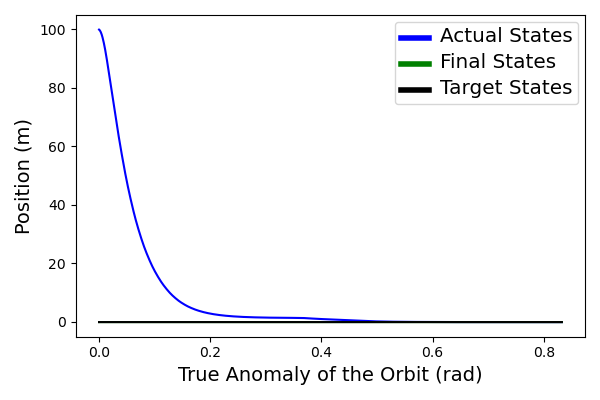
\includegraphics[width=\linewidth]{assets/complete_x_traj.png}
    \caption{Complete Trajectory in the X-axis}
    \label{fig:results_x_rnd}
  \end{subfigure}
  \begin{subfigure}[b]{0.50\textwidth}
    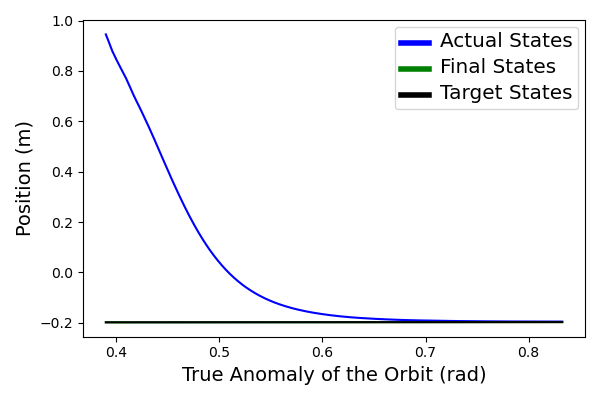
\includegraphics[width=\linewidth]{assets/docking_x_traj.png}
    \caption{Docking Trajectory in the X-axis}
    \label{fig:results_x_dock}
  \end{subfigure}
  \begin{subfigure}[b]{0.50\textwidth}
    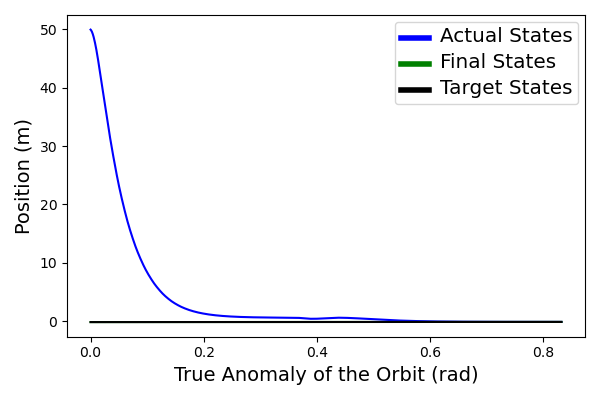
\includegraphics[width=\linewidth]{assets/complete_y_traj.png}
    \caption{Complete Trajectory in the Y-axis}
    \label{fig:results_y_rnd}
  \end{subfigure}
  \begin{subfigure}[b]{0.50\textwidth}
    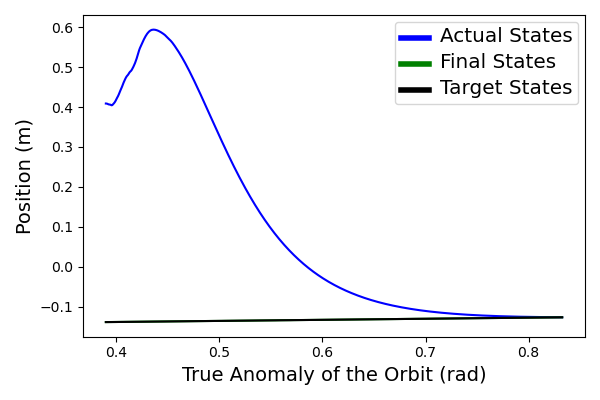
\includegraphics[width=\linewidth]{assets/docking_y_traj.png}
    \caption{Docking Trajectory in the Y-axis}
    \label{fig:results_y_dock}
  \end{subfigure}
  \begin{subfigure}[b]{0.50\textwidth}
    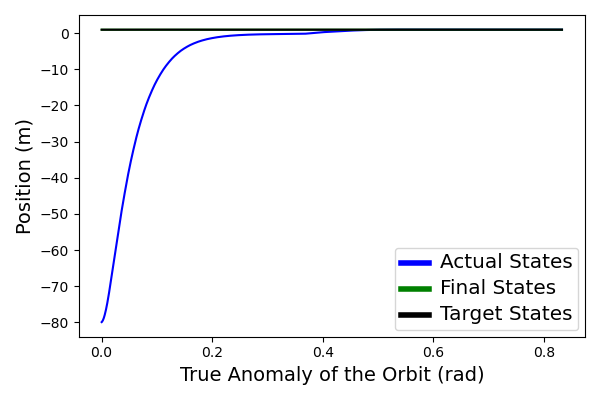
\includegraphics[width=\linewidth]{assets/complete_z_traj.png}
    \caption{Complete Trajectory in the Z-axis}
    \label{fig:results_z_rnd}
  \end{subfigure}
  \begin{subfigure}[b]{0.50\textwidth}
    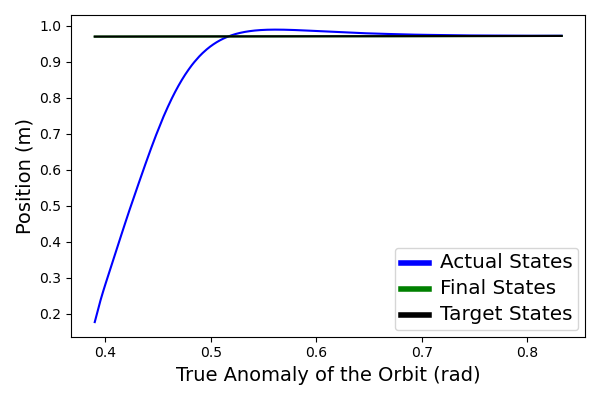
\includegraphics[width=\linewidth]{assets/docking_z_traj.png}
    \caption{Docking Trajectory in the Z-axis}
    \label{fig:results_z_dock}
  \end{subfigure}
  \caption{Simulation of Rendezvous and Docking using ADTMPC}
 \label{fig:results_pipeline}
\end{figure}
The adaptation of the unknown parameters 
- the eccentricity of the orbit and the drag constant of the target - is noted in Table \ref{tab:parameter-estimation} by including the initial and final estimates and ranges of estimation.
We note that it is possible to obtain more precise simulations of the docking operation by adjusting the cost function matrices and other solver parameters; however, we demonstrate the proof-of-concept of the proposed algorithm.
\begin{table}[H]
    \centering
    \resizebox{\textwidth}{!}{\begin{tabular}{|c|c|c|c|c|c|}
    \hline
    Param.                          & Actual Value & Initial Est. & Final Est. & Initial Range & Final Range \\
    \hline
    $\mathsf{e}$         & $\num{1.250e-1}$ & $\num{0.000e-1}$ & $\num{1.2513e-1}$ & $[\num{0.000}, \num{6.000}]\times\num{e-1}$ & $[\num{1.100}, \num{1.373}]\times\num{e-1}$ \\
    $\alpha$ & $\num{1.300e-7}$ & $\num{0.000e-7}$ & $\num{1.2999e-7}$ & $[\num{0.000}, \num{5.000}]\times\num{e-7}$ & $[\num{1.297}, \num{1.326}]\times\num{e-7}$ \\
    \hline
    \end{tabular}}
    \caption{{Estimation of Unknown Parameters via SMID.} This table demonstrates the adaptation of the system to unknown parameters (orbit eccentricity $\mathsf{e}$ and target drag constant $\alpha$) and the shrinking of the estimation ranges.}
    \label{tab:parameter-estimation}
\end{table}
\begin{figure}[H]
  \begin{subfigure}[b]{0.50\textwidth}
    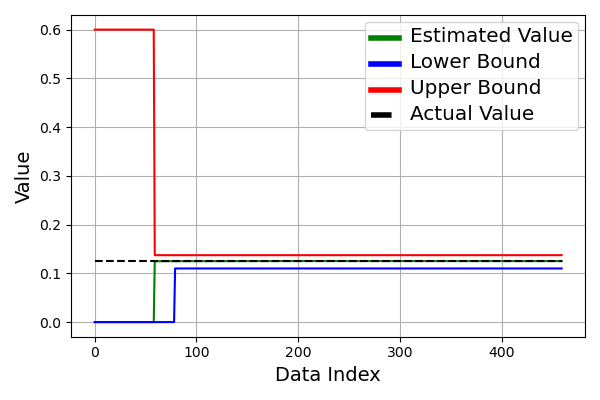
\includegraphics[width=\linewidth]{assets/estim_eccentricity.png}
    \caption{Eccentricity $\mathsf{e}$ of the Orbit}
    \label{fig:results_estim_eccentricity}
  \end{subfigure}
  \hfill
  \begin{subfigure}[b]{0.50\textwidth}
    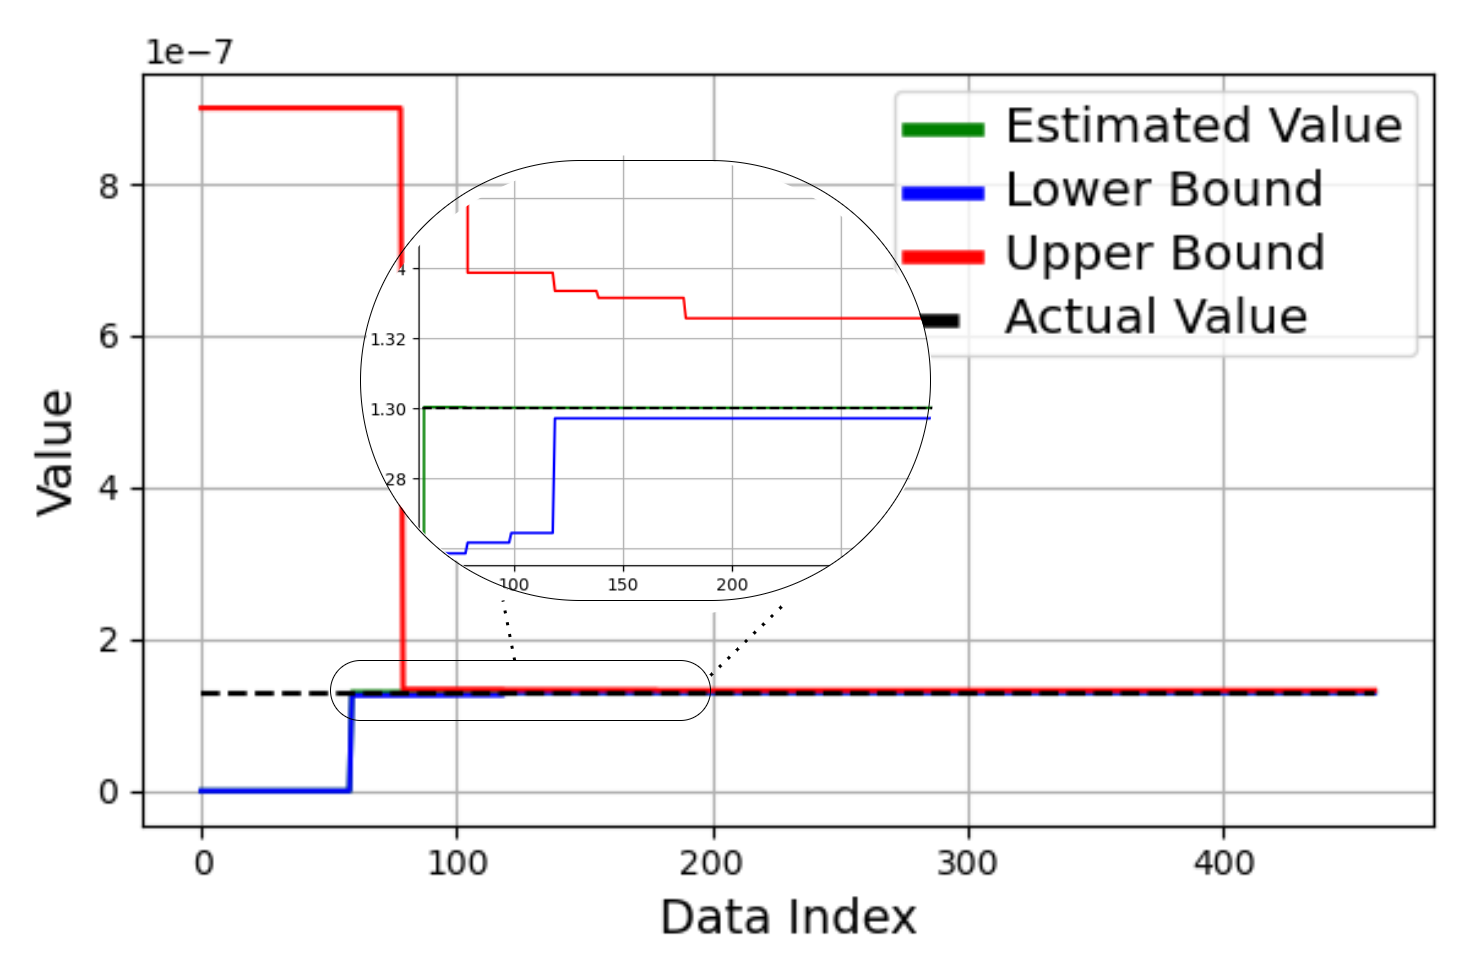
\includegraphics[width=\linewidth]{assets/estim_alpha.png}
    \caption{Drag Constant $\alpha$ of the Target}
    \label{fig:results_estim_alpha}
  \end{subfigure}
  \caption{Estimation of Unknown Parameters via SMID. These figures represent the progress in the estimation of unknown parameters over time using data from the previous MPC iteration.}
  \label{fig:results_estim}
\end{figure}
\subsection{Estimation of Unknown Parameters}
The data in Table \ref{tab:parameter-estimation} and the corresponding plots in Figure \ref{fig:results_estim} demonstrate the estimation of the eccentricity of the orbit and the drag constant of the target from an initial estimate and range to a final estimate that is close to the actual value.
This improves the docking of the chaser due to the corresponding shrinking of the robust tube around the trajectory.
We determine the range and value for eccentricity based on common values of eccentricity for low earth orbits \cite{space2023}.
On the other hand, since this is not easily for target drag constants in orbit, we determine a range and value for this parameter using calculations based on the expression for drag constant and its relation to the standard drag equation \cite{carter2008two,humi2007two}:
\begin{equation}
    F_d=\frac{1}{2}\rho u^2c_dA
\end{equation}
where $F_d$ is the drag force, $\rho$ is the mass density of the fluid, $u$ is the flow velocity relative to the object (in orbit, this can be interpreted as the velocity of the spacecraft), A is the reference area, and $c_d$ is the drag coefficient.

\section{Analysis of ADTMPC and other techniques}
\label{sec:results_analysis}
We perform the following analysis to depict the advantages of using ADTMPC over plain MPC for rendezvous and docking with space debris.
\subsection{Satisfaction of chaser-target collision constraints}
As is visible from Figure \ref{fig:results_tube}, model predictive control without the use of robust tubes leads to the violation of the chaser-target collision constraints in close proximity to the target.
The chaser's trajectory is not able to accurately account for the uncertainties in the target's dynamics and the environment.
In contrast, dynamic tubes help adapt to these uncertainties and maintain a safe distance between the chaser and the target at all times.
\begin{figure}[H]
  \begin{subfigure}[b]{0.49\textwidth}
    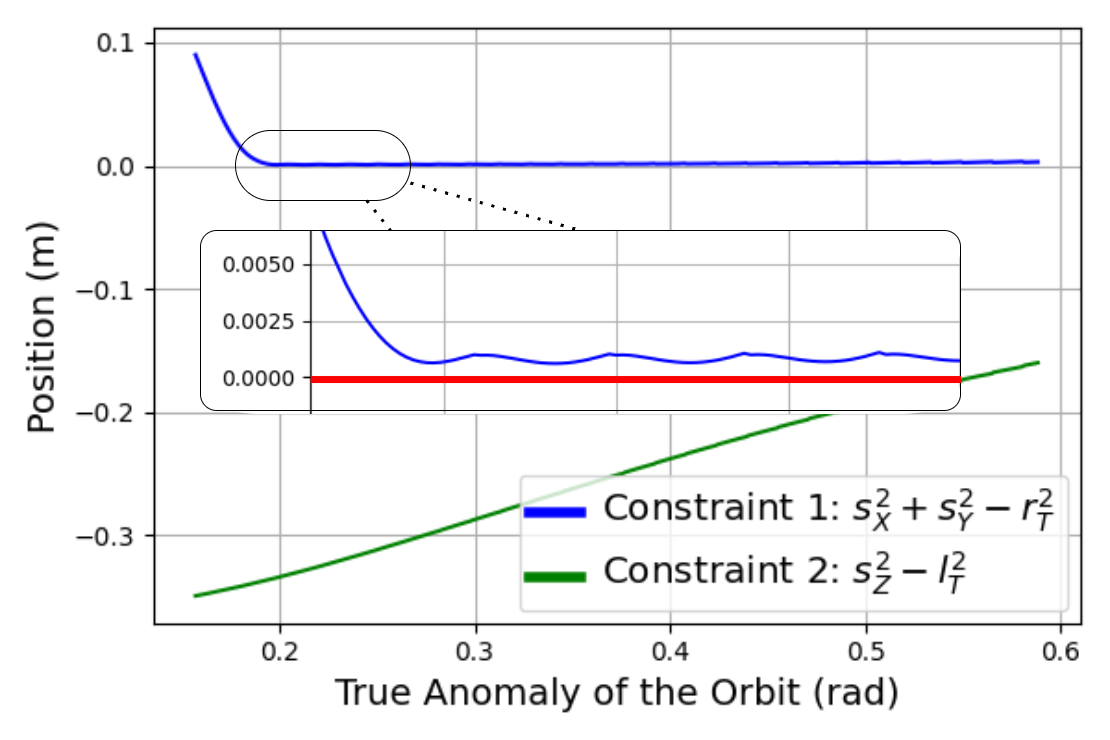
\includegraphics[width=\linewidth]{assets/results_with_tube_dtmpc.png}
    \caption{Dynamic Tube MPC}
    \label{fig:results_with_tube_dtmpc}
  \end{subfigure}
  \hfill
  \begin{subfigure}[b]{0.49\textwidth}
    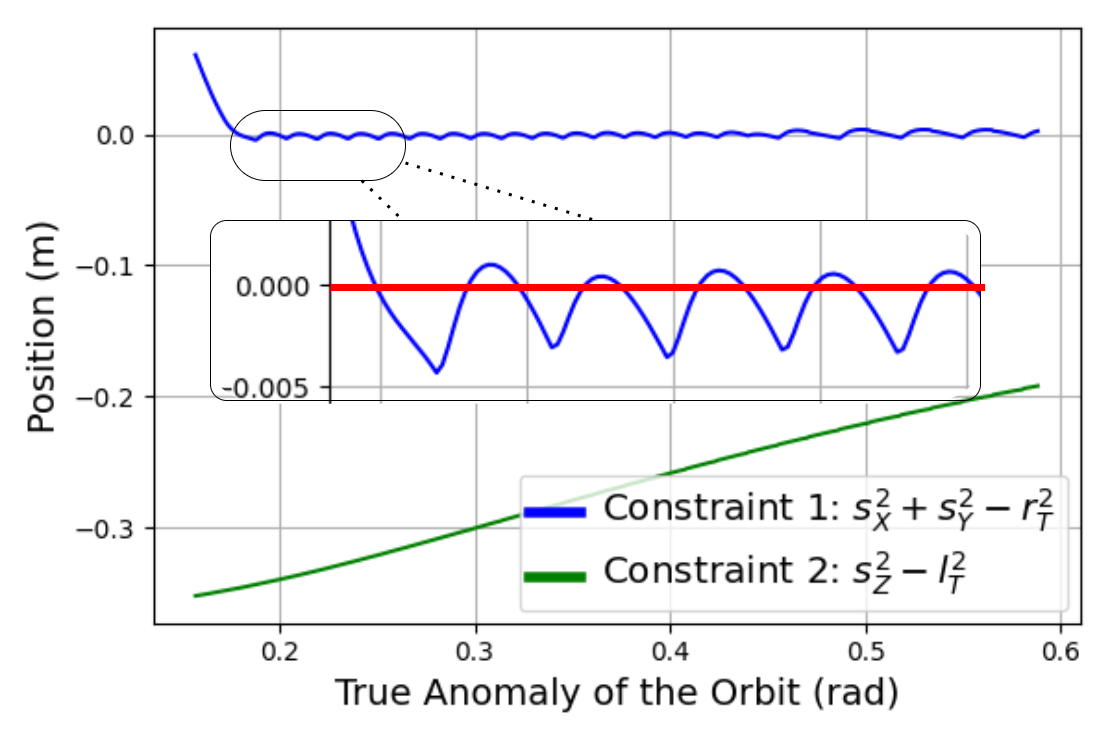
\includegraphics[width=\linewidth]{assets/results_no_tube_mpc.png}
    \caption{MPC (no robust tubes)}
    \label{fig:results_no_tube_mpc}
  \end{subfigure}
  \caption{Violation of Collision Constraints without Robust Tubes. With no robust tubes, there are several time periods when the collision constraint defined as $\boldsymbol{r}(\theta)\in{\mathcal{C}}_D$ is violated; i.e. when both Constraint 1 and Constraint 2 are less than zero.}
  \label{fig:results_tube}
\end{figure}
\subsection{Convergence to the desired docking position}
Although using dynamic tubes without adaptation proves to be effective in preventing collisions, the chaser is unable to converge to the desired docking position on the target due to inaccurate estimates of the unknown parameters and, hence, large robust tubes.
On the other hand, adaptive dynamic tube MPC shrinks the tube over time, hence allowing the chaser to converge to the final docking position.
Figure \ref{fig:results_adapt} demonstrates how, in very close proximity of the chaser to the target, the previous adaptation of unknown parameters and, hence, a smaller robust tube permits the chaser to move closer to the docking position.
\begin{figure}[H]
  \begin{subfigure}[b]{0.50\textwidth}
    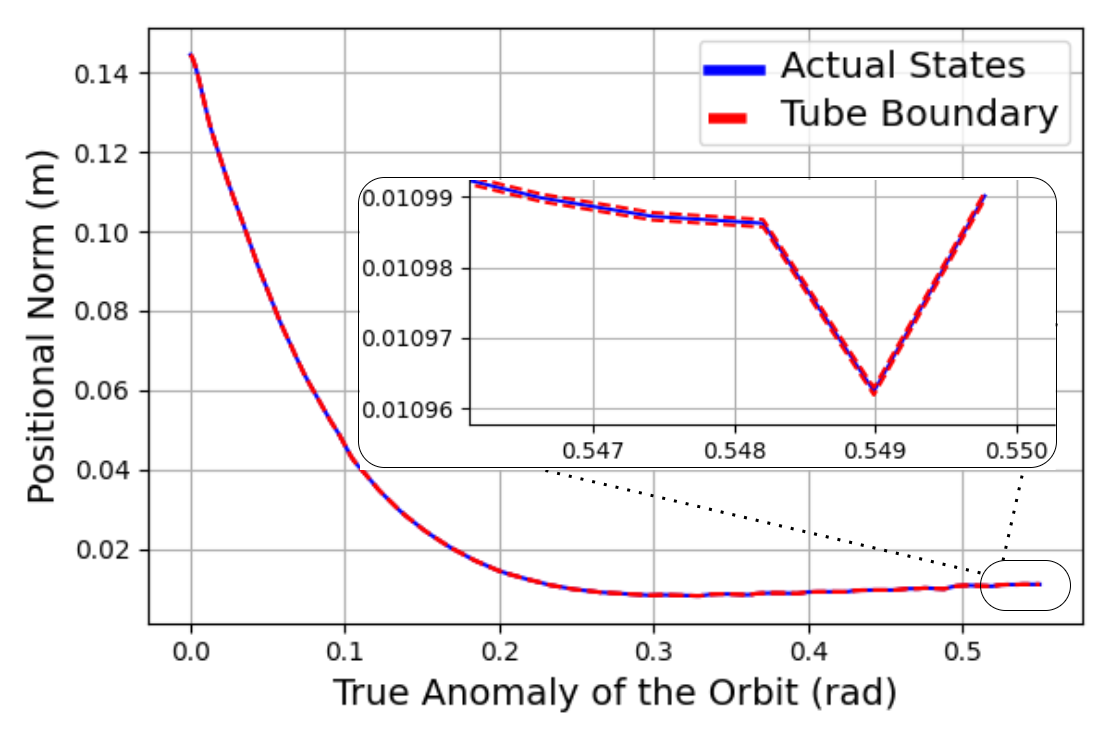
\includegraphics[width=\linewidth]{assets/results_adapt_adtmpc.png}
    \caption{Adaptive Dynamic Tube MPC}
    \label{fig:results_adapt_adtmpc}
  \end{subfigure}
  \hfill
  \begin{subfigure}[b]{0.50\textwidth}
    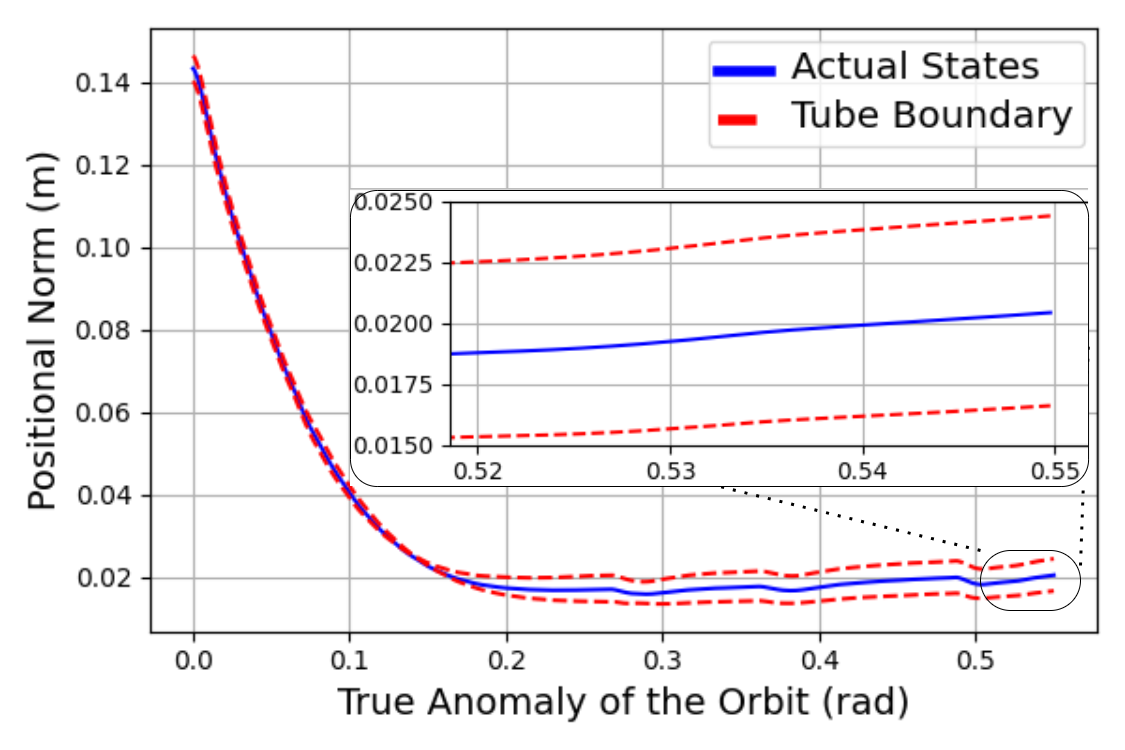
\includegraphics[width=\linewidth]{assets/results_adapt_dtmpc.png}
    \caption{Dynamic Tube MPC (no adaptation)}
    \label{fig:results_adapt_dtmpc}
  \end{subfigure}
  \caption{The Effect of Adaptation. These plots demonstrate the effect of SMID-based parameter estimation on the size of tubes and, hence, the convergence of the chaser to the final docking point.}
  \label{fig:results_adapt}
\end{figure}

\section{Target Deflection}
\label{sec:results_target_deflect}
Next, we run the optimization problem proposed in Section \ref{sec:target-deflection} such that the chaser attaches to a point within a set of known docking positions and applies a net optimal force to detumble the target.
We consider the target to be cylindrical in shape with a non-zero starting angular velocity.
The blue dot in figures \ref{fig:results_docking_point_unrestricted} (for the case with unrestricted docking points) and \ref{fig:results_docking_point_discretized} (for the case with discretized docking points) represents the optimal position of docking of the chaser on the target.
This point has been optimally calculated from a set of 24 points, 8 uniformly distributed on each circular boundary and 8 on the circle halfway between the boundary circles.
Figures \ref{fig:results_deflection_unrestricted} and \ref{fig:results_deflection_discretized} further demonstrate the trajectories of the angular position and the angular velocity of the target, and the forces applied by the chaser to stop its tumble.
\begin{table}[H]
    \centering
    \resizebox{\textwidth}{!}{\begin{tabular}{|c|c|c|c|}
        \hline
        & $\boldsymbol{\omega}_i$ (rad/s) & $\boldsymbol{\omega}_f$ (rad/s) & $||\boldsymbol{\omega}_f||$ (rad/s) \\
        \hline
        Unrestricted & $[-0.04, 0.10, -0.02]$ & $[\num{-9.614e-6}, \num{6.835e-6}, \num{-1.293e-7}]$ & $\num{1.180e-5}$ \\
        Discretized  & $[-0.04, 0.10, -0.02]$ & $[\num{-2.844e-3}, \num{7.571e-2}, \num{-2.402e-2}]$ & $\num{7.947e-2}$ \\
        \hline         
    \end{tabular}}
    \caption{Target Detumbling using Unrestricted and Discretized Docking Points}
    \label{tab:target_detumbling}
\end{table}
\begin{figure}[H]
  \centering
  \begin{subfigure}[b]{0.4\textwidth}
    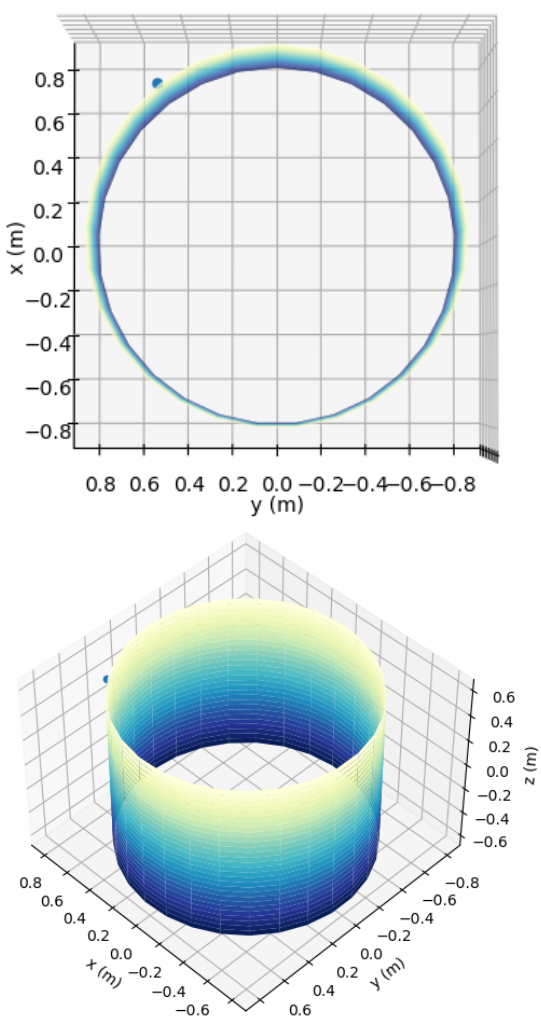
\includegraphics[width=\linewidth]{assets/results_docking_point_unrestricted_vert.png}
    \caption{Unrestricted Docking Points}
    \label{fig:results_docking_point_unrestricted}
  \end{subfigure}
  \begin{subfigure}[b]{0.4\textwidth}
    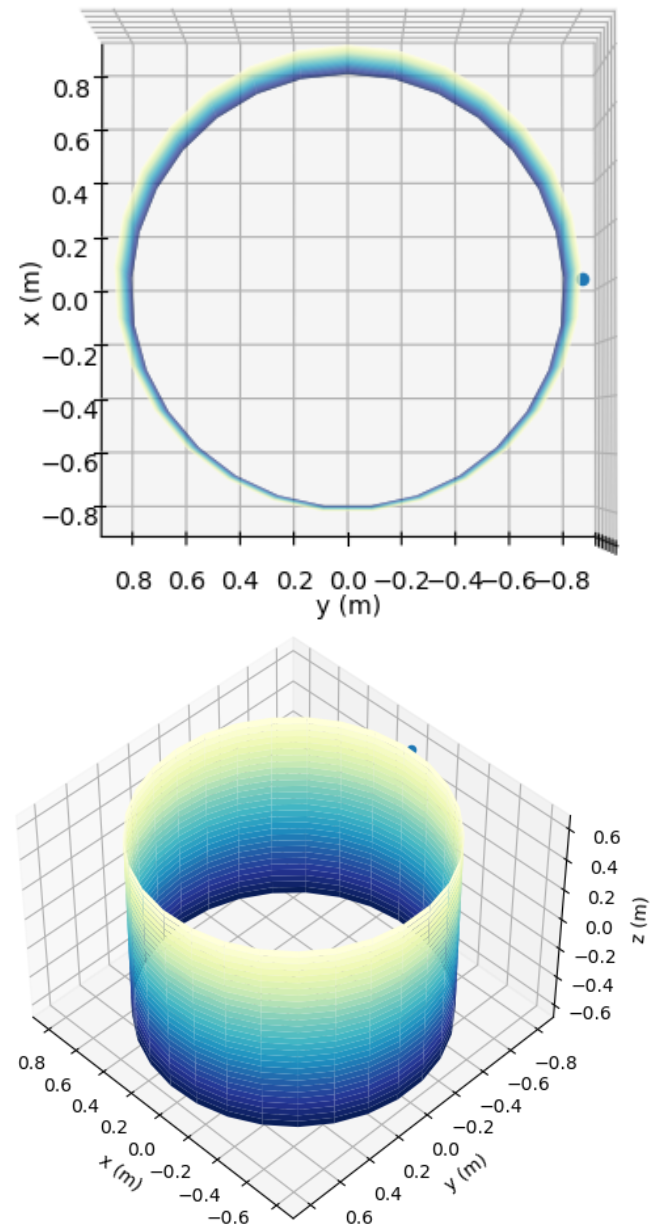
\includegraphics[width=\linewidth]{assets/results_docking_point_discretized_vert.png}
    \caption{Discretized Docking Points}
    \label{fig:results_docking_point_discretized}
  \end{subfigure}
  \caption{Optimal Chaser Docking Position}
  \label{fig:results_docking_point}
\end{figure}
It can be observed from Table \ref{tab:target_detumbling} that, with no restriction on the docking position of the chaser, the angular velocity of the target is brought to zero, hence stopping the tumble of the target.
The angular velocity of the target is significantly decreased even with discretized docking points.
This is also reflected in the convergence of the target angular position.
The unrestricted case provides a globally optimal position for docking whereas the discretized case picks the most optimal position from a finite set (in this case, a set of 48 points) which need not be the globally optimal position.
As a result, the force required to detumble the target is significantly larger for the latter case.
The docking positions are also different due to the discretization process and the subsequent difference in the initialization of the nonlinear dynamic optimization problem.
\section{Summary}
This chapter presents results on the simulation of rendezvous and docking of a single chaser with a cylindrical target in an elliptical orbit with drag.
It is shown that the implementation of dynamic tubes for robustness prevents inevitable collision with the target. 
Furthermore, the chapter demonstrates the accuracy of estimating the eccentricity of the orbit and the drag constant of the target.
This subsequently shrinks the robust tube around the trajectory of the chaser, hence making the trajectory less conservative.
Finally, the chapter presents results on the deflection of the target using chaser propulsion, comparing results for when any point on the target can be chosen for docking against the case with a discrete set of docking positions.
While the former case provides a globally optimal solution bringing the target to a standstill, the latter also significantly decreases the tumble of the target.
% \begin{figure}[H]
%     \centering
%     \includegraphics[width=0.95\linewidth]{assets/results_docking_point_unrestricted.png}
%     \caption{Optimal Chaser Docking Position with Unrestricted Docking Points}
%     \label{fig:results_docking_point_unrestricted}
% \end{figure}
% \begin{figure}[H]
%     \centering
%     \includegraphics[width=0.95\linewidth]{assets/results_docking_point_discretized.png}
%     \caption{Optimal Chaser Docking Position with Discretized Docking Points}
%     \label{fig:results_docking_point_discretized}
% \end{figure}


% UNRESTRICTED
% Position of the Chaser:  [0.63453837 0.49735406 0.6       ]
% Initial Angular Position: [ 0.0 0.2 -0.1 ]
% Initial Angular Velocity: [ -0.04 0.1 -0.02 ]
% Final   Angular Position: [ -0.0015024259646 0.20362891089 -0.10051285282 ]
% Final   Angular Velocity: [ -9.6140430806e-06 6.8354931586e-06 -1.2926002949e-07 ]
% Norm of Initial Angular Velocity:  0.10954451150103323
% Norm of Final   Angular Velocity:  1.1797054684628867e-05

% DISCRETIZED
% Position of the Chaser:  [-1.48628994e-06 -8.00000616e-01  6.00000240e-01]
% Initial Angular Position: [ 0.0 0.2 -0.1 ]
% Initial Angular Velocity: [ -0.04 0.1 -0.02 ]
% Final   Angular Position: [ -0.020816099278 0.22113934686 -0.058538949531 ]
% Final   Angular Velocity: [ -0.002844002 0.075705397522 -0.024016434397 ]
% Norm of Initial Angular Velocity:  0.10954451150103323
% Norm of Final   Angular Velocity:  0.07947442785252029
\begin{figure}[H]
  \centering
    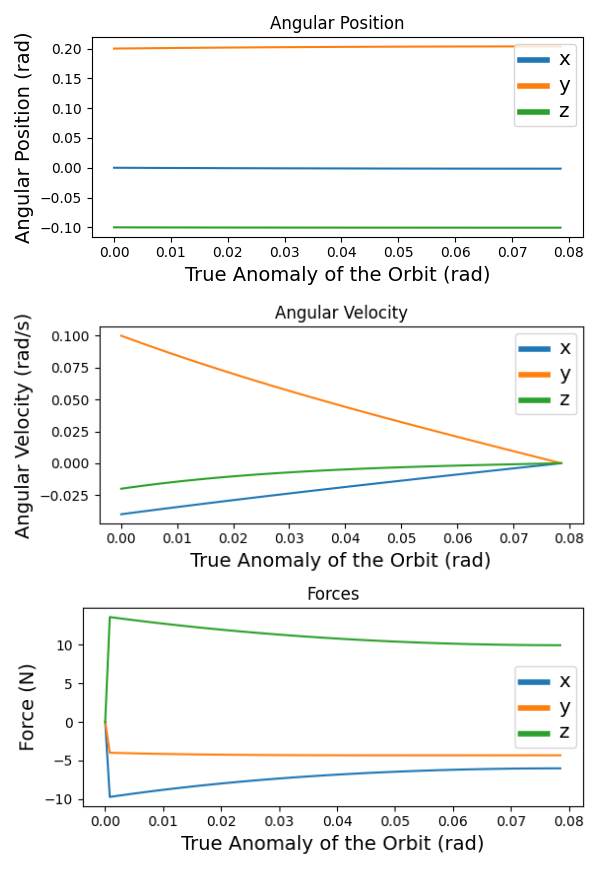
\includegraphics[width=0.8\linewidth]{assets/target_output_unrestricted.png}
  \caption{Detumbling of the Target and the Corresponding Chaser Control Effort with Unrestricted Docking Points.}
  \label{fig:results_deflection_unrestricted}
\end{figure}
\begin{figure}[H]
  \centering
    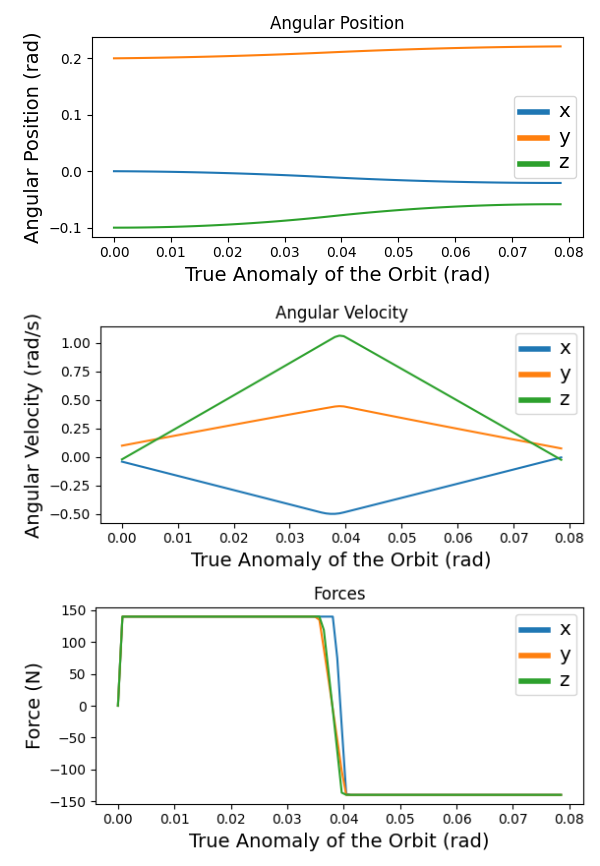
\includegraphics[width=0.8\linewidth]{assets/target_output_discretized.png}
  \caption{Detumbling of the Target and the Corresponding Chaser Control Effort with Discretized Docking Points.}
  \label{fig:results_deflection_discretized}
\end{figure}
\chapter{Conclusion}
\label{ch:conclusion}
In this thesis, we propose a novel approach to the problem of autonomous detumbling of non-cooperative tumbling objects in orbit using adaptive dynamic tube model predictive control (ADTMPC).
Our approach addresses the issue of unknown parameters during the operation such as the eccentricity of the orbit and the drag constant of the target.
Our approach is based on parameter estimation using set membership identification in concurrence with optimal trajectory planning for rendezvous and docking.
We further utilize robust control-invariant tubes to prevent collision violations in spite of uncertainties.
We also suggest how this can be extended to a multi-agent solution in consideration of larger targets.
Finally, we propose the logic behind detumbling the target after docking.
We have evaluated our approach on a simulated scenario involving a single chaser performing rendezvous and docking with a tumbling object in low Earth orbit.
The results show that our approach is able to successfully rendezvous, dock, and deflect the tumbling object.

We plan to extend our work and suggest future work in the implementation of a multi-agent solution including the possibility for extended observation in different directions by different chasers permitting the collection of more information over shorter time frames.
Stricter constraints for docking as suggested in Appendix \ref{app:conical-constraints} can be introduced in order to support faster and more efficient docking.
We also suggest future work in the realm of multi-target interaction where there arises the need to interact and detumble heterogeneous targets in close proximity with each other (hence posing an imminent threat of cross-collision) and with the chasers.
% \appendices{}
\appendix

\chapter{Relative Motion in a Circular Orbit with No Drag} \label{app:cwh-equations}
This appendix references \cite{clohessy1960terminal} to describe the motion of a chaser in close proximity to a target in a circular orbit with no drag.
The translational dynamics of the chaser are described using the Clohessy-Wiltshire-Hill (CWH) Equations as follows:
\begin{subequations}
\begin{align}
    \frac{d^2x}{dt^2}&=2n\frac{dy}{dt},\\
    \frac{d^2y}{dt^2}&=-2n\frac{dx}{dt}+3n^2y,\\
    \frac{d^2z}{dt^2}&=-n^2z,
\end{align}
\end{subequations}
where the x-axis points radially into the Earth (opposite to the radius vector of the target spacecraft), the z-axis is along the angular momentum vector of the target spacecraft, and the x-axis completes the right-handed system.
Here,
\begin{align}
    n&=\sqrt{\frac{\mu}{a}},
\end{align}
where $\mu=GM_E$ is the standard gravitational parameter for the Earth as the central body (geocentric gravitational constant) and $a$ is the radius of the target's orbit.
This can be rewritten as a linear time-invariant (LTI) system:
\begin{equation}
    \dot{\boldsymbol{r}}(t)=A\boldsymbol{r}(t)+B\boldsymbol{u}(t),
\end{equation}
where
\begin{subequations}
\begin{align}
    \boldsymbol{r}(t)&=\begin{bmatrix}
    x(t)&y(t)&z(t)&\dot{x}(t)&\dot{y}(t)&\dot{z}(t)
    \end{bmatrix}^T,\\
    \boldsymbol{u}(t)&=\begin{bmatrix}
    u_x(t)&u_y(t)&u_z(t)
    \end{bmatrix}^T,\\
    A&=\begin{bmatrix}
        0_{3\times3}&I_{3\times3}\\
        n^2A_{\dot{r}r}&nA_{\dot{r}\dot{r}}
    \end{bmatrix},\\
    B&=\begin{bmatrix}
        0_{3\times3}\\
        I_{3\times3}
    \end{bmatrix},
\end{align}
\end{subequations}
such that:
\begin{subequations}
\begin{align}
    A_{\dot{r}r}&=\begin{bmatrix}
        0&0&0\\
        0&3&0\\
        0&0&-1
    \end{bmatrix},\\
    A_{\dot{r}\dot{r}}&=\begin{bmatrix}
        0&2&0\\
        -2&0&0\\
        0&0&0
    \end{bmatrix}.
\end{align}
\end{subequations}

\chapter{Relative Motion in an Elliptical Orbit with Quadratic Drag} \label{app:ellp-undrag}
This appendix references \cite{carter2002clohessy} to describe the motion of a chaser with respect to the local-vertical-local-horizontal frame of reference of the target in an elliptical orbit with quadratic drag (considering the possibility of unequal drag constants between the chaser and the target). Considering the position, velocity, control input, and other quantities to now be in terms of the true anomaly $\theta$ of the orbit and $\theta_0$ is the initial true anomaly of the orbit such that:
\begin{subequations}\begin{align}
    \boldsymbol{r}(\theta)&=\begin{bmatrix}
    x(\theta),y(\theta),z(\theta),x'(\theta),y'(\theta),z'(\theta)
    \end{bmatrix}^T,\\
    \boldsymbol{u}(\theta)&=\begin{bmatrix}
    u_x(\theta),u_y(\theta),u_z(\theta)
    \end{bmatrix}^T,
\end{align}
\end{subequations}
the dynamics of the chaser are given as:
\begin{equation}
    \boldsymbol{r}'(\theta)=A(\theta,\theta_0)\boldsymbol{r}(\theta)+B\boldsymbol{u}(\theta)+\boldsymbol{d}(\theta, \theta_0),
\end{equation}
where
\begin{subequations}
\begin{align}
    A(\theta, \theta_0)&=\begin{bmatrix}
        0_{3\times3}&I_{3\times3}\\
        A_{r'r}(\theta, \theta_0)&A_{r'r'}(\theta, \theta_0)
    \end{bmatrix},\\
    B&=\begin{bmatrix}
        0_{3\times3}\\
        I_{3\times3}
    \end{bmatrix},\text{ and}\\
    d(\theta, \theta_0)&=\begin{bmatrix}
        0_{3\times1}\\
        R(\theta,\theta_0)d_i(\theta,\theta_0)\\
        -R'(\theta,\theta_0)d_i(\theta,\theta_0)\\
        0
    \end{bmatrix},
\end{align}
\end{subequations}
such that:
\begin{subequations}
\begin{align}
    A_{r'r}&=\begin{bmatrix}
        -\gamma\frac{R'}{R}&\gamma&0\\
        -\gamma&-\gamma\frac{R'}{R} + \frac{3Re^{2\alpha\theta}\mu}{h^2}&0\\
        0&0&-1-\gamma\frac{R'}{R}
    \end{bmatrix},\\
    A_{r'r'}&=\begin{bmatrix}
        -\gamma&2&0\\
        -2&-\gamma&0\\
        0&0&\gamma
    \end{bmatrix},
\end{align}
\end{subequations}
and the new quantities dependent on eccentricity and drag constants are defined as
\begin{subequations}
\begin{align}
    \gamma&= \beta - \alpha,\\
    d_i(\theta,\theta_0) &= \frac{\gamma R(\theta,\theta_0)e^{\alpha\theta}}{\sqrt{h}},\\
    R(\theta,\theta_0) &= \frac{h^2(1+4\alpha^2)}{\mu} \frac{1}{e^{2\alpha\theta} + {\mathsf{e}}\cos{(\theta - \theta_0)}},\\
    R'(\theta,\theta_0)&=\frac{dR}{d\theta}(\theta,\theta_0),
\end{align}
\end{subequations}
where ${\mathsf{e}}$ is the eccentricity of the orbit of the target, $\theta$ is the true anomaly of the orbit of the target, $\alpha$ is the drag constant of the target, and $\beta$ is the drag constant of the chaser.
We point the reader to observe the equivalence of this system to the CWH equations provided in Appendix \ref{app:cwh-equations} when the eccentricity of the orbit and the drag constants of both the target and the chaser are all set to zero.

We draw a parallel between the drag equation provided in the paper:
\begin{equation}
    \boldsymbol{a}_{D}=-\frac{\alpha}{R}|\dot{\boldsymbol{R}}|\dot{\boldsymbol{R}},
\end{equation}
where $\boldsymbol{R}$ is the position of the satellite from the center of the Earth and $R=|\boldsymbol{R}|$, and the standard drag equation \cite{batchelor2000an}
\begin{equation}
    F_{D}=\frac{1}{2}\rho v^{2}C_{D}A,
\end{equation}
where $F_{D}$ is the drag force, $\rho$ is the density of air, $v$ is the speed of the chaser, $A$ is the cross-sectional area, and $C_{D}$ is the dimensionless drag coefficient of the chaser to deduce that $\alpha$ and $\beta$ lie in the range of $10^{-7}$ \cite{li2011perturbation}.
This is used in preparing the setup for the results we present in Chapter \ref{sec:results}.

\chapter{The Minimum Enclosing Ellipsoid of the Target}
\label{app:mee}
We consider the minimum enclosing ellipsoid (MEE) \cite{kallberg2019minimum} of the target to be a pseudo-target of radii $a$, $b$, and $c$.
Let T be a set of points on the target that minimally defines the complete boundary of the target.
The minimum enclosing ellipsoid of the target can be defined as:
\begin{align}
    \frac{x^2}{a^2}+\frac{y^2}{b^2}+\frac{z^2}{c^2}&=1,
\end{align}
where $a$, $b$, and $c$ can be computed using the following minimization problem:
\begin{equation}
\begin{aligned}
    \min_{a, b, c}\quad &V=\frac{4}{3}\pi abc\\
    \textrm{s.t. } & a,b,c>0,\\
    & \frac{p_x^2}{a^2}+\frac{p_y^2}{b^2}+\frac{p_z^2}{c^2}<1.\quad\forall\ p\in \text{T}
    \label{eqn:mee}
\end{aligned}
\end{equation}

\chapter{Conical Constraints for Docking}
\label{app:conical-constraints}
We suggest the addition of a conical constraint:
\begin{align}
    f_{\text{cone}}(\bm{r}(t), \bm{r}_d, \alpha)<0, \label{eqn:conical-constraint}
\end{align}
to ensure safe docking in the final docking approach phase. The function $f_{cone}$ can be defined as:
\begin{align}
    f_{\text{cone}}(\bm{r}(t), \bm{r}_d, \alpha)=\left(\bm{r}(t)-\bm{r}_d\right)\cdot\bm{r}_d-\frac{||\bm{r}(t)-\bm{r}_d||\ ||\bm{r}_d||}{\sqrt{1-\alpha^2}}.
\end{align}
However, this can be linearized by constructing two hyperplanes that define the edges of the entry cone and intersect at the docking point as described in \cite{park2017nonlinear}.
We propose adapting the aperture $2\phi$ of the conical constraint to modify aggressiveness in docking and, hence, the ratio of the radius to the height $\alpha=\tan\phi$ as:
\begin{align}
    \alpha&=f_\alpha\left(\left|\frac{\theta_e}{\hat{\theta}}\right|\right),
\end{align}
where $\theta$ is the actual value of the unknown parameter (here, the goal docking position of the chaser), $\hat{\theta}$ is the estimated value of the parameter, and $\theta_e=d(\theta,\hat{\theta})$ is the error in estimation, such that:
\begin{align}
    f_\alpha(x) =           0 & \text{ if } x = 0,\\
    f_\alpha(y) > f_\alpha(x) & \text{ if } y > x.
\end{align}
% For example, we consider the following relation (for practicality, we keep $\alpha$ small but non-zero when the error in estimation is zero):
% \begin{align}
%     \alpha&=\exp{\left(\left|\frac{\theta_e}{\hat{\theta}}\right|\right)}-1.
% \end{align}
% \bibliography {bib/network,bib/naming}
\bibliography{include/biblio.bib}
% \bibliographystyle {thesis}
\bibliographystyle{uclathes}

\end{document}